

%!TEX root = ./main.tex
%** Results.tex: What were the results achieved including an evaluation
\chapter{Results and Evaluation 
\label{chapter:results}}

This chapter covers the an detailed analysis of a one-week long monitoring of server sockets in section \ref{section:analysis_in_wild}.
This data used for this analysis is briefly described in section \ref{section:data}.
Their statistical characteristics with respect to stability, visibility and popularity are examined. 

Furthermore, an evaluation of the traffic preselection of \gls{FACT} based on server sockets and the effect on \gls{FACT}'s observation capabilities is done in section \ref{section:enhanced_FACT_eval}.

Finally, section \ref{section:results} briefly summarizes the main findings of this chapter. 

\todo{Write introduction}

%%%%%%%%%%%%%%%%%%%%%%%%%%%%%%%%%%%%%%%%%%%%%%%%%%%%%%%%%%%%%%%%%%%%%%%%%%%%%%%%
% DATA
%%%%%%%%%%%%%%%%%%%%%%%%%%%%%%%%%%%%%%%%%%%%%%%%%%%%%%%%%%%%%%%%%%%%%%%%%%%%%%%%
\section{Data 
\label{section:data}}

This thesis relies on data collected at \citet{switch}, the Swiss National Research and Education Network (NREN). 
Mainly government institutions, universities, research labs are connected to the Internet by \citet{switch}\citep{Schatzmann:Mining}.

The \citet{switch} network is with approximately 250'000 network users in 2010 comparable with a mid sized \gls{isp}. Currently, there are around 2.4 million \gls{IPv4} addresses, a /32 IPv6 and a /40 \gls{IPv6} network announced via \gls{bgp}\citep{Schatzmann:Tracing}.
\begin{figure}
	[ht] \centering 
	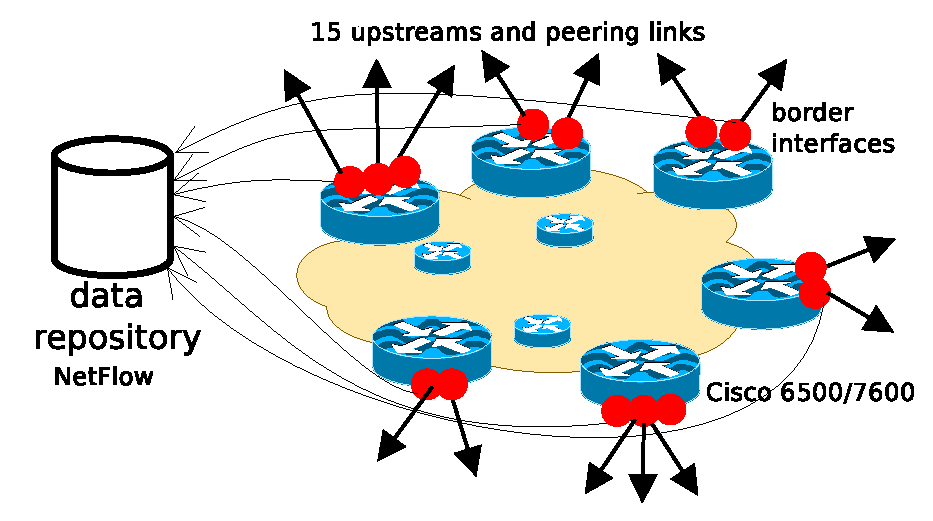
\includegraphics[width=12cm]{images/network_overview.eps} \caption{Overview of the SWITCH network \citep{SchatzmanThesis2012}} 
	\label{fig:switch_nework} 
\end{figure}

Figure \ref{fig:switch_nework} provides an overview of the SWITCH network. 
Currently, SWITCH has 15 upstreams and peering links and is capturing flow level data at all external interfaces of their border routers. From 2003 to 2008 to version 5 has been used, and version 9 after 2008\citep{Schatzmann:Tracing}.

High traffic peak rates of more than 80'000 flows per second, 3 million packets per second and more than 20Gbit/s require hardware-based flow collection cards\citep{Schatzmann:Tracing}. 
\gls{TCP} flags are not available in the flow-level information because of limitations of the used hardware components\citep{Schatzmann:Tracing}. 
The generated flow data are collected and stored in a central data repository.

% briefly describe the Switch network and its topology..
% traffic volume and netflow data unsampled!
% see tech report 338 for numbers and layout?! evtl actual numbers (2012)
%%%%%%%%%%%%%%%%%%%%%%%%%%%%%%%%%%%%%%%%%%%%%%%%%%%%%%%%%%%%%%%%%%%%%%%%%%%%%%%%
%%%%%%%%%%%%%%%%%%%%%%%%%%%%%%%%%%%%%%%%%%%%%%%%%%%%%%%%%%%%%%%%%%%%%%%%%%%%%%%%
% ANALYSIS of SERVER SOCKETS IN THE WILD
%%%%%%%%%%%%%%%%%%%%%%%%%%%%%%%%%%%%%%%%%%%%%%%%%%%%%%%%%%%%%%%%%%%%%%%%%%%%%%%%\newpage
\section{Analysis of Server Sockets in the Wild\label{section:analysis_in_wild}}

This section covers an analysis of \gls{server socket} found during a week long data trace from 2010/11/01 00:00:00 UTC until 2010/11/06 00:49:00 UTC, thus covering mainly the first 5 working days in November 2010.

\subsection{Detected Server Sockets}

% sum up of detection parameters > 2 biflows per 5min interval with more TCP
% packets > 3 UDP > 1
For detecting the \glspl{server socket} in this observation period, the previously discussed detection approach was applied as illustrated by figure \ref{fig:detection_chain}. 
In detail, the connection cache was configured with a cache interval of 600 seconds and an export interval of 300 seconds. Hence, all flows active during the last 600 seconds are exported every 300 seconds. The cache interval of 600 seconds is chosen according to \citet{Schatzmann:Tracing} for making it likely to observe at least some flows to any active server socket. 

%to summarize all related unidirectional flow records into a single bidirectional flow record during an aggregation interval of 600s.
After this caching step, these bidirectional flows are filtered by a fan-out filter implementing the idea of \citet{Allman:2007} to mitigate the effects of scanning and \gls{p2p} churn. 
This fan-out filter is configured to require at least 4 unidirectional connections with a certain host as source and at least 2 times more unidirectional connections than bidirectional connections for classifying this host as a scanning host. 
Previous work\citep{Schatzmann:Mining,Schatzmann:Dissection, Schatzmann:Tracing} has shown that these parameters are a good choice for efficiently mitigating the scanning noise so that the scanning spikes of the total traffic volume are successfully reduced.

Moreover, the noise filter is configured to filter all bidirectional \gls{TCP} flows with less than 3 packets in a single direction and bidirectional \gls{UDP} flows which are actually unidirectional flows and have 0 packet in a single direction.

Furthermore, the \emph{server socket detector} is configured to extract sockets with a degree of 2 or higher as concentrators, thus requiring two independent connections to a \gls{server socket} within 600 seconds.

% state overall number of detected external and internal server sockets during
% this period
During the entire observation period of 120.8 hours, the \emph{server socket detector} managed to detect 1'862'389 external \glspl{server socket} and 609'670 internal \glspl{server socket}.

\subsection{Traffic Attraction of Server Sockets}

% traffic statistics of server sockets detected by type and ratio of traffic
% towards server sockets
In the following, the overall traffic statistics of the detected \glspl{server socket} are briefly discussed. Figure \ref{fig:flows_by_type} shows the absolute number of flows during the entire observation period separated by the type of connection. 
If the flow is destined to a \gls{server socket}, the flow is denoted as monitored, otherwise as unmonitored. 
Furthermore, the type of connection also considers the balance or direction of the connection, i.e.,if the flow is bidirectional, unidirectional outgoing or unidirectional incoming. 
Hence, in total there are 6 possible combinations for the type of connection, allowing a good interpretation of the detection approach. 
For easier comparison of each type of connection, figure \ref{fig:monitored_flows_by_type} shows the ratio of monitored and unmonitored flows by the direction.

In figures \ref{fig:flows_by_type} and \ref{fig:monitored_flows_by_type}, there are two gaps visible around 2010/11/01 10:00 UTC and 2010/11/04 06:05 UTC. 
These gaps result from missing flow records due to router reboots, collector outages, and storage failures\citep{Schatzmann:Mining}.
\begin{figure}
	[ht] \centering 
	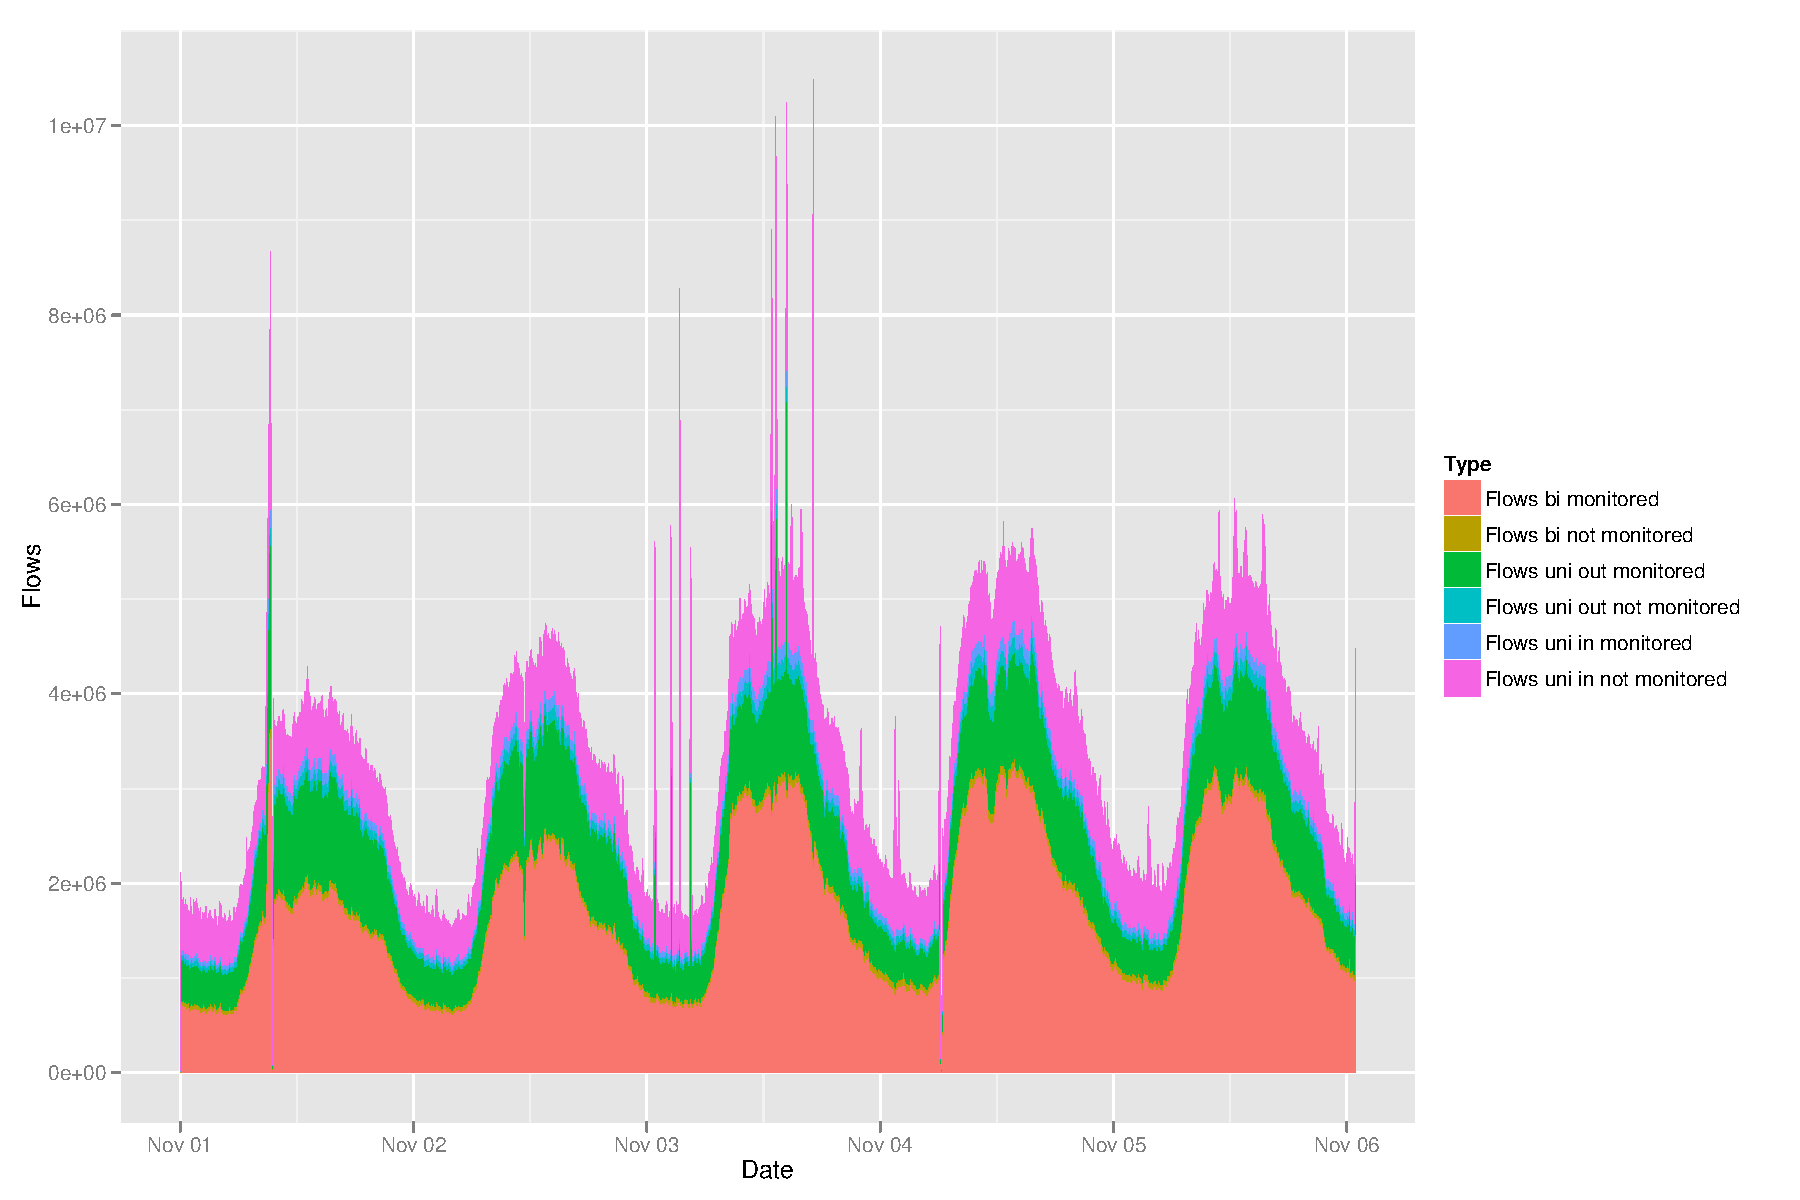
\includegraphics[width=\linewidth]{images/Flows_by_type_area_all_SeS.pdf} \caption{Number of flows over time by the type of connection with all detected server sockets} 
	\label{fig:flows_by_type} 
\end{figure}
\begin{figure}
	[h] \centering 
	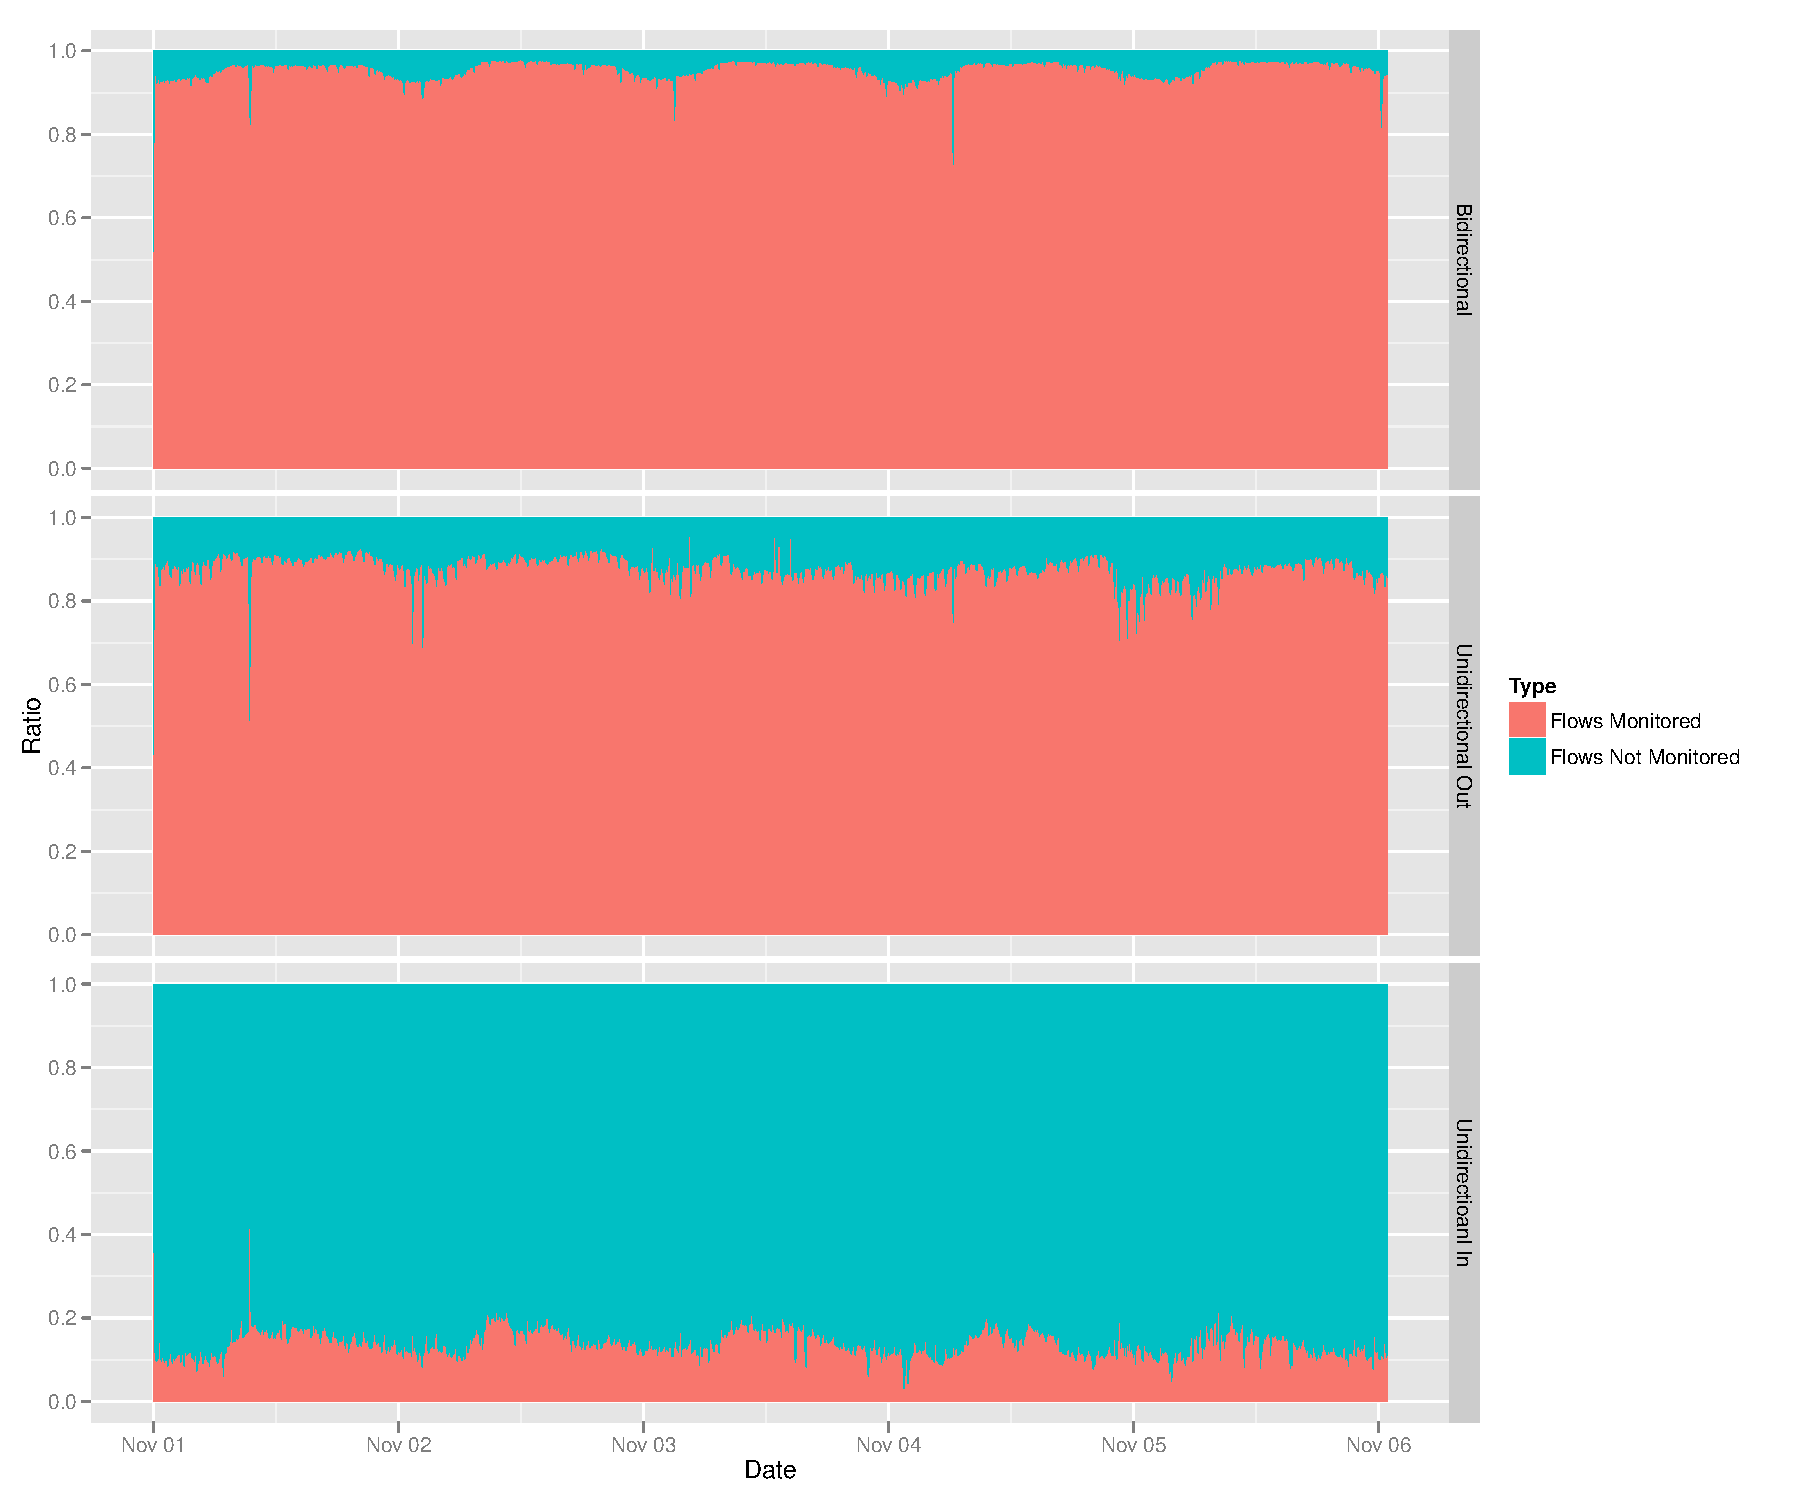
\includegraphics[width=\linewidth]{images/Flows_monitor_ratio_by_type_all_SeS.pdf} \caption{Flows towards known server sockets by traffic type with all detected server sockets} 
	\label{fig:monitored_flows_by_type} 
\end{figure}

Clearly, the dominating kind of the flows are the bidirectional monitored flows represented by the red area in figure \ref{fig:flows_by_type}. 
Comparing this share with the bidirectional unmonitored flows represented by the hardly visible yellow\todo{CHANGEME! IF figure \ref{fig:monitored_flows_by_type}} area between the red and the green area, yields that the detection approach detects a majority of the \glspl{server socket}. 
This finding is even better visible on the bidirectional ratio of figure \ref{fig:monitored_flows_by_type}. 
Depending on the time of the day, the monitoring ratio of the bidirectional flows is mainly between 90\% and 97\%. 
The smaller monitoring ratios during night indicates that there is a higher share of unknown \glspl{server socket} active at night than during day. 
A possible reason for pattern is that there are some \glspl{server socket} which are regularly contacted, although, only by very few clients so that these sockets get never more than one connection within 600 seconds. 
Thus, these sockets are never detected as concentrators.

Similarly, if the unidirectional outgoing flows are examined by looking at figure \ref{fig:monitored_flows_by_type}, the monitored flows have predominantly a high share of around 80\% to 90\% of all unidirectional outgoing flows. 
Figure \ref{fig:flows_by_type} also reveals some high peaks which are probably scanning or backscatter effects which are well visible at November 03 in the night and in the afternoon by the green spikes. 
However, these green peaks are categorized as monitored unidirectional outgoing flows. 
Thus, they must involve at least one known \gls{server socket} either located external or internal.

Finally, the unidirectional incoming flows have are predominately unmonitored with around 80-97\% of unmonitored flows as it can be seen in figure \ref{fig:monitored_flows_by_type}. 
The main reason for this contrast may be that the main part of this unidirectional incoming traffic consists of Internet background radiation \citep{Wustrow10,Pang04} due to malware or misconfiguration for example. 
Nevertheless, this unidirectional incoming flow traffic is unimportant with respect to the scope of this thesis.

To sum up, \glspl{server socket} tend to attract a majority of the observed connections, especially the bidirectional connections and the unidirectional connections which are important to the connectivity tracking. 
Therefore, they are well suitable to represent legitimate traffic which is interesting for tracking the end-to-end connectivity.

%In a metaphorical sense, \glspl{server socket} are comparable to masses in physics which are exerting gravitational forces to other objects. 
%\Glspl{server socket} tend to attract a majority of the observed connections. 
%Therefore, they are well suitable to represent a majority of the legitimate traffic which is interesting for tracking the end-to-end connectivity.
\newpage 
\subsection{Characterization of Detected Server Sockets}

As discussed in section \ref{section:characterization}, this thesis proposes to characterize \glspl{server socket} according to their visibility, popularity and stability by different metrics. This section aims to deduce some statistical properties of the detected \glspl{server socket} regarding these characteristics.

\subsubsection{General Visibility of Server Sockets}

For defining a metric of the visibility of \glspl{server socket}, it is required to define the granularity of a observation period according to \ref{subsection:visibility}. For simplicity reasons, only two different granularities are defined.

One the one hand, a day long observation period yields the number of visible days for the activity of a socket. 
On the other hand, an observation period of 5 minutes is chosen, since it reflects the default processing interval of FlowBox and the native caching interval of the flow data. 
This allows a very fine-grained, detailed resolution of a \glspl{server socket} activity. 
This second visibility metric is referred as \emph{visible time slots(VTS)}.
\begin{figure}
	[hb] \centering 
	\includegraphics[width=\linewidth]{images/VTS_by_visibledays.pdf} \caption{Each of the six histogram shows the number of sockets by visible time slots for the corresponding visible days} 
	\label{fig:vts_by_visibledays} 
\end{figure}

Figure \ref{fig:vts_by_visibledays} shows six histograms. Each of the histograms shows the visible time slots of the sockets separated by their daily visibility. This means that the histogram of all sockets with a daily visibility 1 day is the top left diagram. \todo{Describe me better!?!} The skewness of the distributions for 1 to 4 visible days are is very similar. 
It is obvious that the a socket which is visible for only one day cannot exceed 288 visible time slot. 
Nonetheless, considering this daily scaling factor, the distributions are looking very similar. 
Furthermore, figure \ref{fig:vts_by_visibledays} shows that the most sockets in absolute terms are only active during one day and only in very few visible time slots.

However, the distribution of the number of sockets with a visibility of 5 or even 6 days are slightly different, since there is a higher share of sockets with a relatively higher visible time slots, besides the normal scaling factor of the number of visible days. \todo{CONCLUSION!}

\subsubsection{Visibility and Stability} Eventually, for selecting those \glspl{server socket} which are stable and often visible it is of importance to assess how \glspl{server socket} are distributed with respect to their stability and visibility characteristic. 
Hence, figure \ref{fig:rankedVisibility} shows the quantile of the visible time slot of each socket and their stability. 
Thus, a socket with a visibility quantile of 80\% indicates that there are 80\% of all sockets with the same or lower visibility than this specific socket.

As figure \ref{fig:rankedVisibility} indicates, the sockets cluster around the top right corner, hence the top visible sockets tend to have a good stability as well. \todo{CONCLUSION!}
\begin{figure}
	[hb] \centering 
	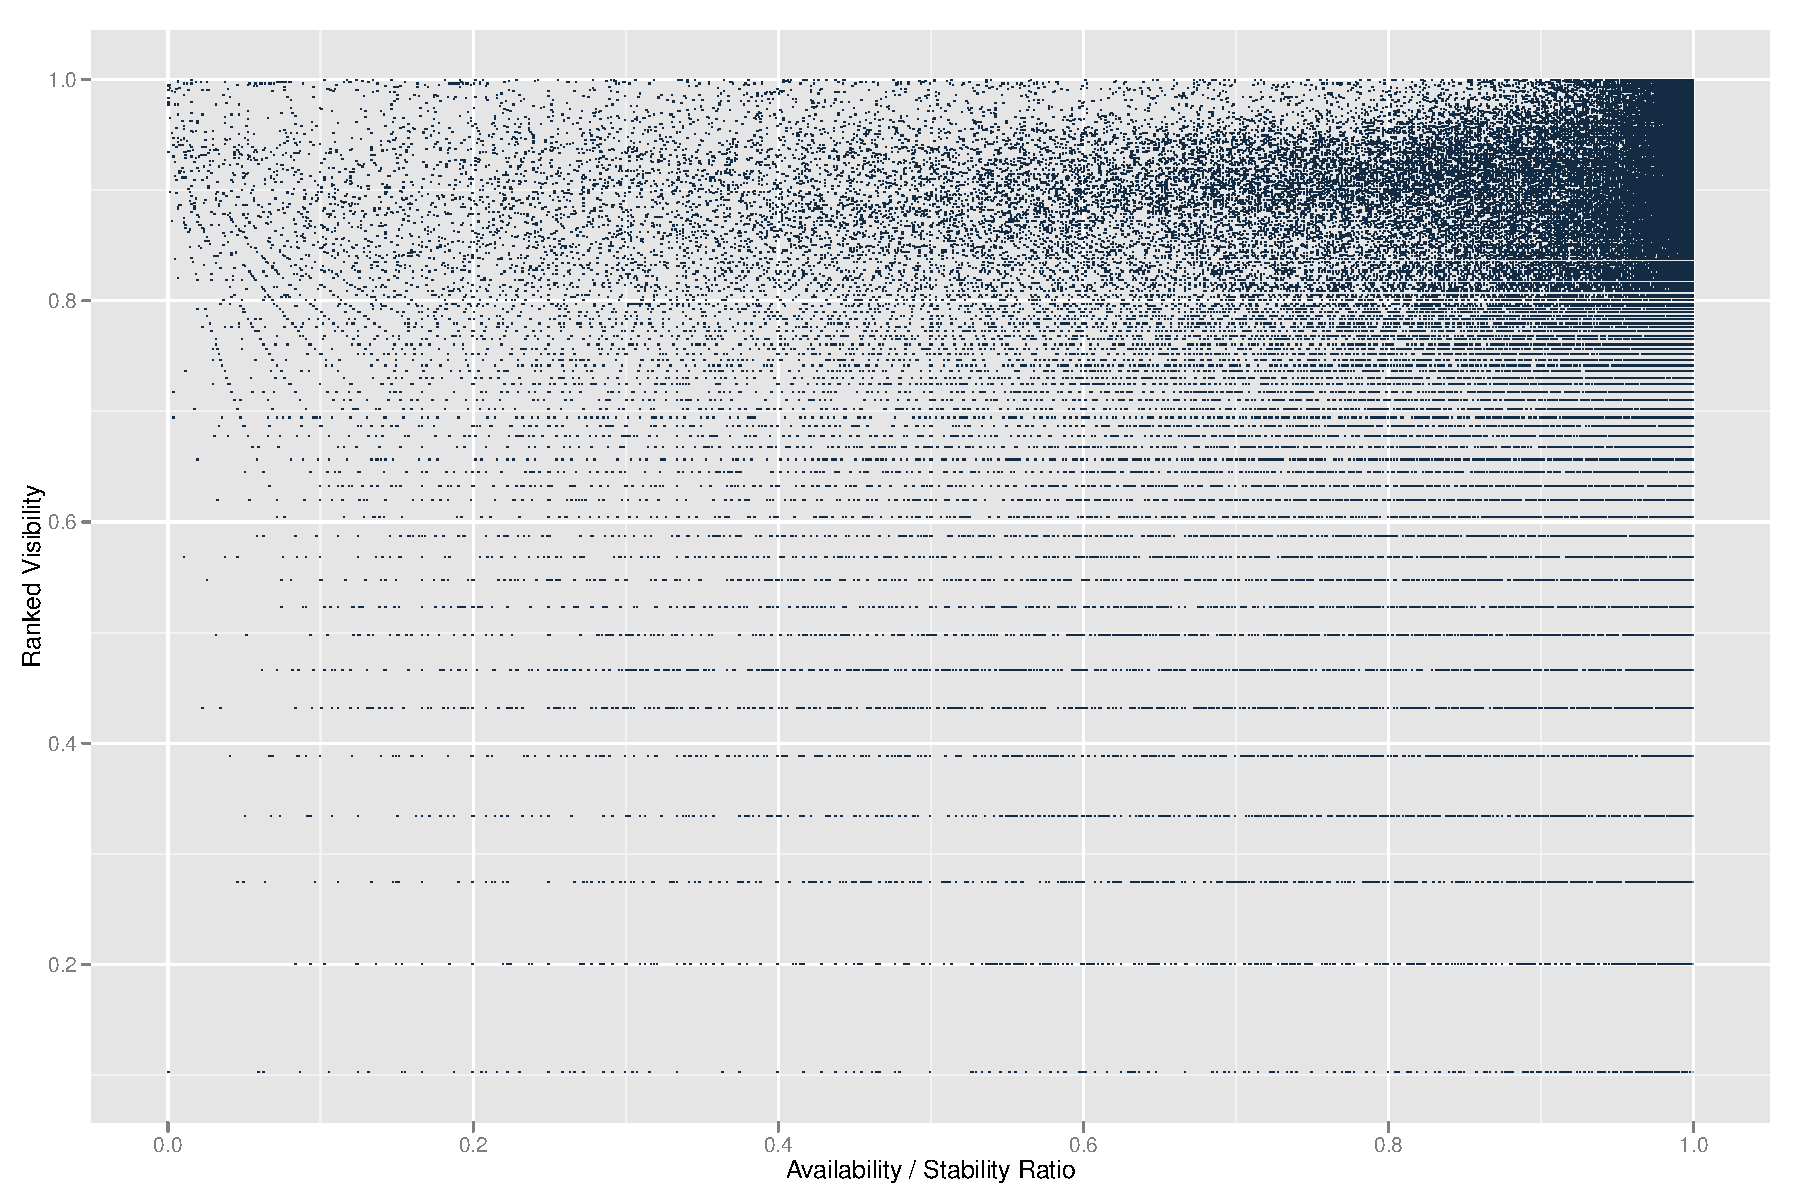
\includegraphics[width=\linewidth]{images/visibiliy_stability_map.pdf} \caption{Quantiles of the visible time slots of each socket and the corresponding stability stability} 
	\label{fig:rankedVisibility} 
\end{figure}

Furthermore, figures \ref{fig:ccdf_ratio_days} and \ref{fig:ccdf_ratio_vts} show each a complementary cumulated distribution function of the stability of server sockets with different visibilities.

One the one side, figure \ref{fig:ccdf_ratio_days} is using the daily visibility of the sockets. 
The red curve represents the distribution of the sockets which are seen only in one day. 
Not surprisingly, these group of \glspl{server socket} reveal the highest share of sockets with a stability of 1. 
This is mainly due to the fact that there is a high number of \glspl{server socket} which are active only during a relatively short period of time. This can be justified by looking at figure \ref{fig:vts_by_visibledays}.

Not surprisingly there is a higher share of sockets with a visibility of 2 days with a stability ratio below 80\%. 
Intuitively, the sockets which have a good visibility of 5 or even 6 days tend to have a high stability as well, but they have a lower share of sockets which have a stability ratio of 1 than all other. 
This means that sockets which are often visible incline to have at least some unbalanced connections.

On the other side, figure \ref{fig:ccdf_ratio_vts} shows the complementary cumulative distribution function of the stability ratio of sockets with different absolute visible time slots. 
Around 99\% of all \glspl{server socket} with more than 1000 visible time slots have a higher stability ratio than 95\%. 
Although, only around 20\% of them have a stability ratio of 100\%, i.e., they have no unbalanced connections at all. 
As in figure \ref{fig:ccdf_ratio_days}, \glspl{server socket} with a low visibility incline to have a higher share of sockets with a stability ratio below 90\% than sockets more often visible. \todo{CONCLUSION!}
\begin{landscape}
	\begin{figure}
		[p] \centering 
		\includegraphics[width=\linewidth]{images/CCDF_ratio_days.pdf} \caption{CCDF of the availability by visible days} 
		\label{fig:ccdf_ratio_days} 
	\end{figure}
\end{landscape}
\begin{landscape}
	\begin{figure}
		[p] \centering 
		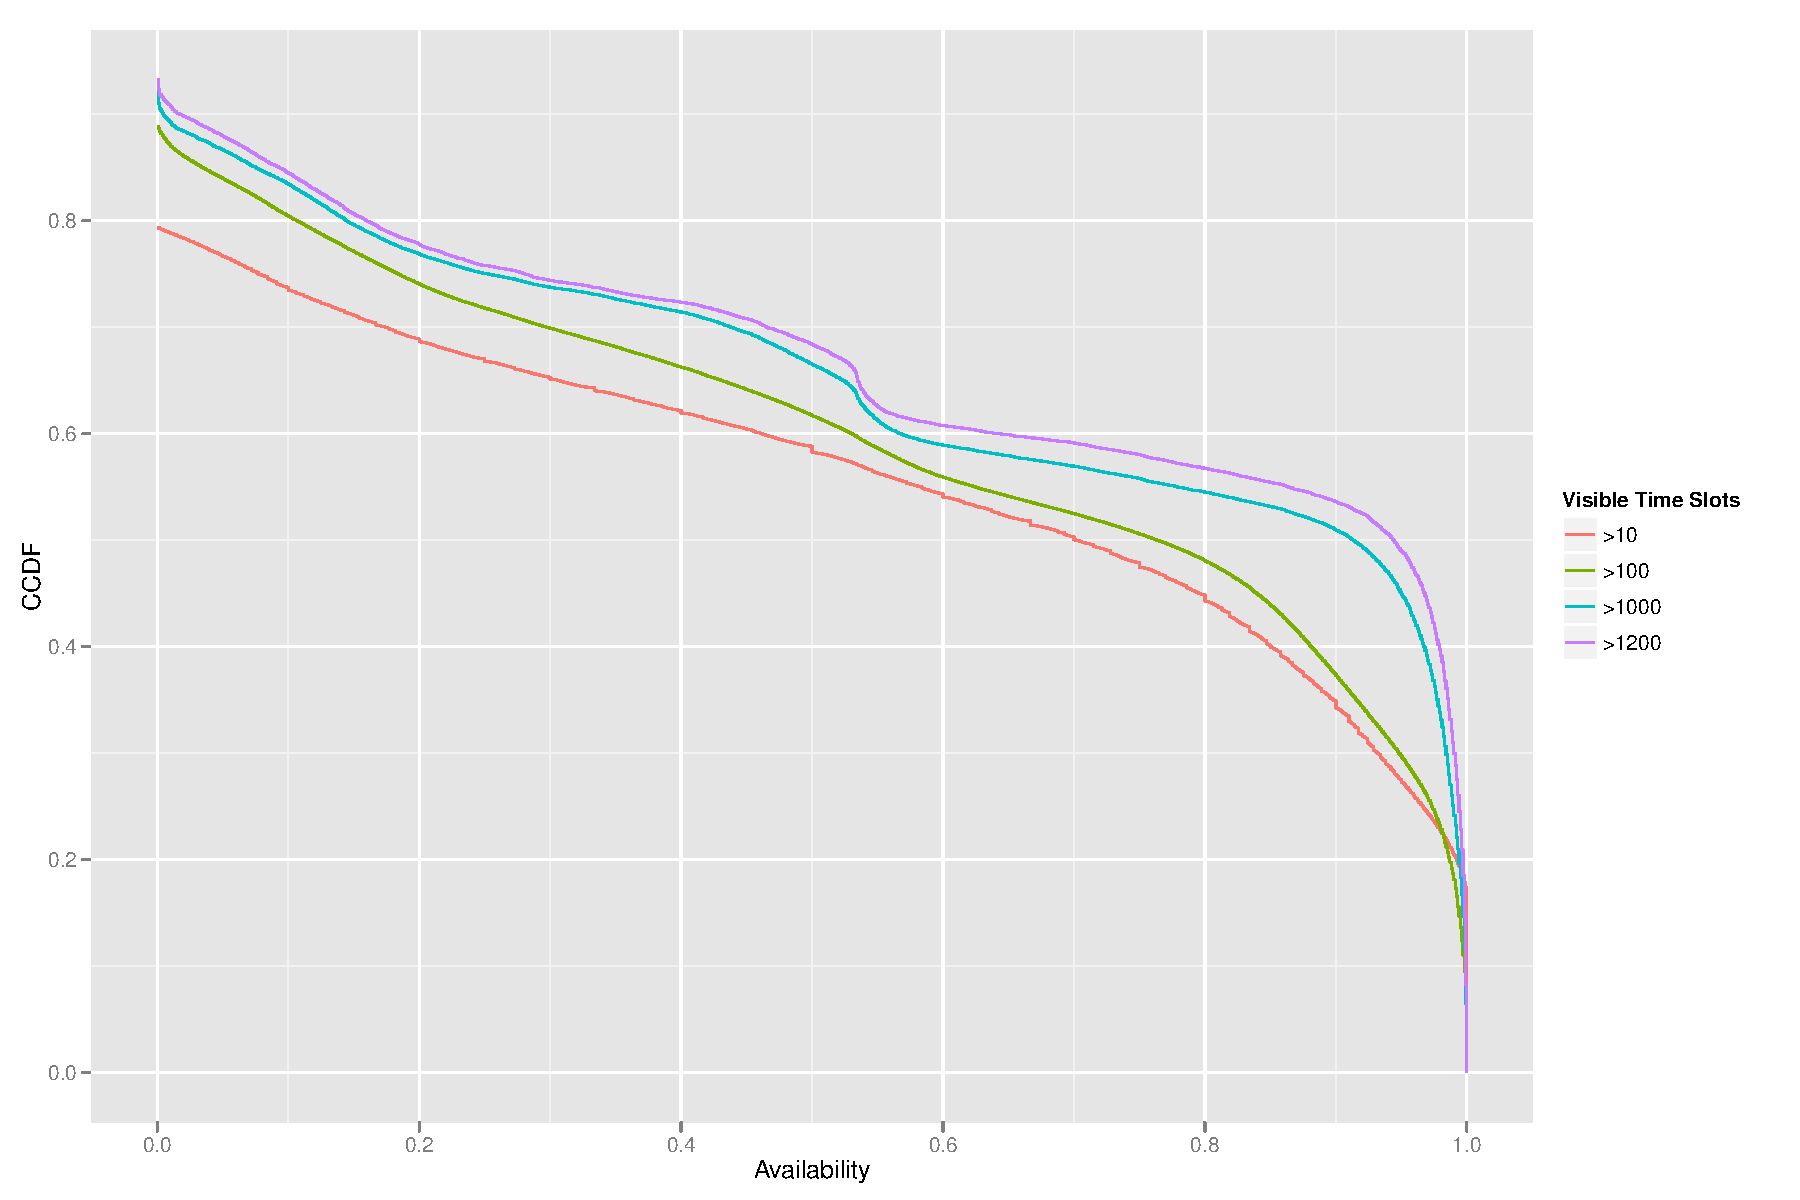
\includegraphics[width=\linewidth]{images/CCDF_ratio_VTS.pdf} \caption{CCDF of the availability by visible time slots} 
		\label{fig:ccdf_ratio_vts} 
	\end{figure}
\end{landscape}

\subsubsection{Popularity and Stability} Similarly to the visibility, the \glspl{server socket} characteristics of popularity and stability are briefly assessed in the following. 
For this reason, the ranked popularity is defined in the same way as the ranked visibility. 
To be precise, the ranked popularity is defined as the cumulative distribution function of the popularity in terms of flows. 
Hence, a \gls{server socket} with a ranked popularity of 80\% signifies that there are 80\% of all \gls{server socket} with a lower or equal popularity as this specific socket.

Figure \ref{fig:rankedPopularity} shows the \glspl{server socket} by their ranked popularity and their stability ratio. 
Similarly to figure \ref{fig:rankedVisibility}, the \glspl{server socket} tend to cluster in the top right corner of figure \ref{fig:rankedPopularity}. This indicates that popular sockets tend to have a good stability as well. \todo{CONCLUSION!}
\begin{figure}
	[ht] \centering 
	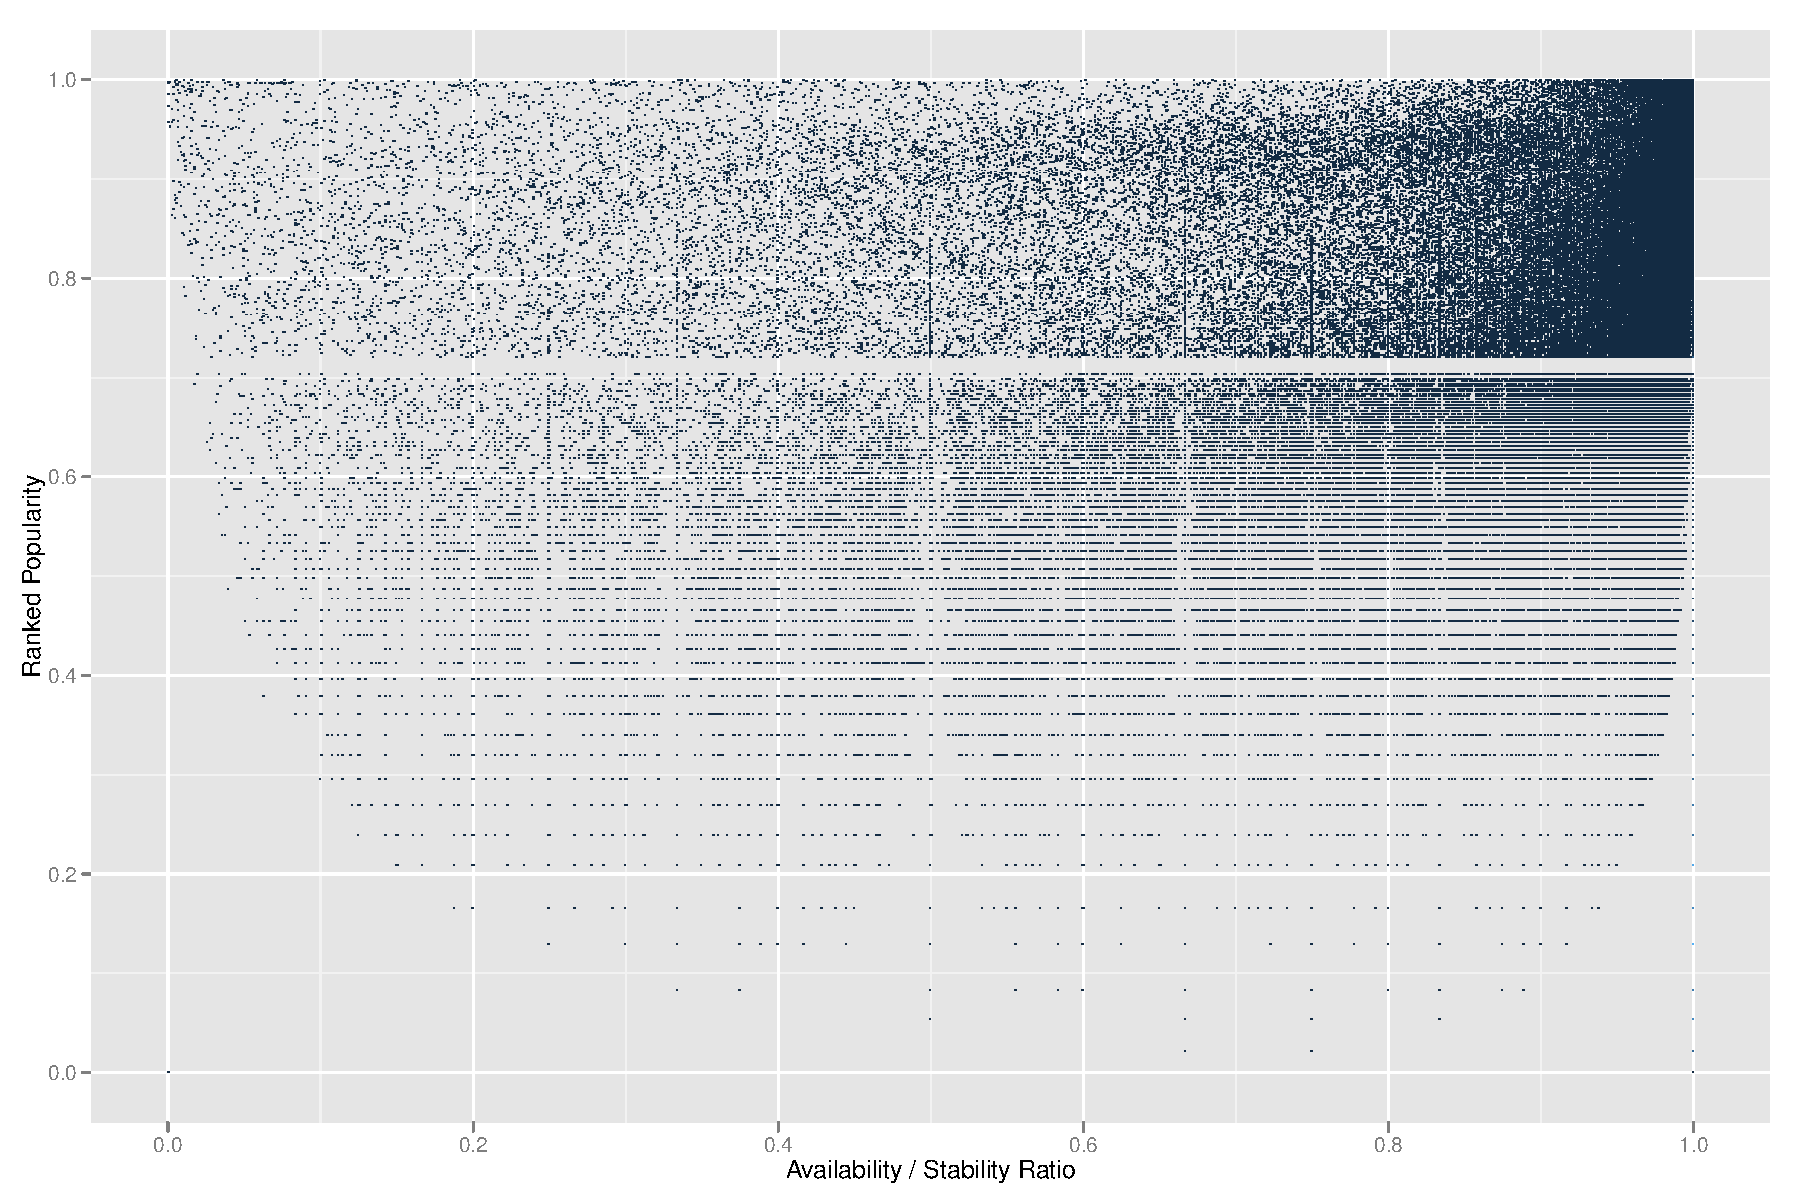
\includegraphics[width=\linewidth]{images/popularity_stability_map.pdf} \caption{Sockets by their ranked popularity and their stability} 
	\label{fig:rankedPopularity} 
\end{figure}

By aggregating all sockets by their protocol and port, some statistical insights can be gained, however, these insights are relative to a port centric view, since it does for example not differentiate the kind of application running on these sockets. 
Nonetheless, some useful information can be gained by comparing individual sockets with these port/protocol aggregated statistics of the same protocol and port. 
Hence, some statements about the characteristics relative to all other sockets can be made.

Basically, figure \ref{fig:top20_ratio_box} shows a box-and-whisker plot of the stability ratio of the 20 most popular ports. 
For most of the ports two box-plots are shown, one for \gls{UDP} in blue, and the other for \gls{TCP} in red. 
A box-and-whisker plot indicated with a box the range from the first quartile to the third quartile, also denoted as hinges, thus indicating where 50\% of all sockets of this kind are located. 
In the middle of the box, the median is illustrated by a black line. 
The whisker is connecting the hinges to the fences which represents the upper and lower extreme value. 
Moreover, some (statistical) outliners below or above the fences are shown by black dots. 
\todo{describe top 20 ports after getting new top 20 results for table}
\begin{landscape}
	\begin{figure}
		[p] \centering 
		\includegraphics[width=\linewidth]{images/top20_ratio_box.pdf} \caption{box-and-whisker plot of the availability / stability of the top 20 traffic port server sockets} 
		\label{fig:top20_ratio_box} 
	\end{figure}
\end{landscape}
\begin{landscape}
	\begin{figure}
		[p] \centering 
		\includegraphics[width=\linewidth]{images/top20_visibility_box.pdf} \caption{box-and-whisker plot of visibility in days of the top 20 traffic port server sockets} 
		\label{fig:top20_visibledays_box} 
	\end{figure}
\end{landscape}
\begin{table}
	[ht] \centering 
	\begin{tabular}
		{|c|r|r|r|r|r|r|} \hline \textbf{Position} & \textbf{Port} & \textbf{Protocol} & \textbf{Flows} &\textbf{ Flows in \%} & \textbf{Sockets} & \textbf{Sockets in \%}\\
		\hline \hline 1 & 53 & 17 & 1026787508 & 46.6799 & 327099 & 17.5634 \\
		\hline 2 & 80 & 6 & 845917736 & 38.4572 & 602008 & 32.3245 \\
		\hline 3 & 443 & 6 & 91197155 & 4.1460 & 67869 & 3.6442 \\
		\hline 4 & 555 & 6 & 10929909 & 0.4969 & 11 & 0.0006 \\
		\hline 5 & 22 & 6 & 10744151 & 0.4885 & 40797 & 2.1906 \\
		\hline 6 & 2703 & 6 & 10141483 & 0.4611 & 23 & 0.0012 \\
		\hline 7 & 25 & 6 & 9478055 & 0.4309 & 20155 & 1.0822 \\
		\hline 8 & 123 & 17 & 7119334 & 0.3237 & 318 & 0.0171 \\
		\hline 9 & 993 & 6 & 4377631 & 0.1990 & 1795 & 0.0964 \\
		\hline 10 & 12043 & 6 & 4002264 & 0.1820 & 294 & 0.0158 \\
		\hline 11 & 995 & 6 & 3157801 & 0.1436 & 962 & 0.0517 \\
		\hline 12 & 110 & 6 & 2808154& 0.1277 & 1662 & 0.0892 \\
		\hline 13 & 6005 & 6 & 2530274 & 0.1150 & 15 & 0.0008 \\
		\hline 14 & 53 & 6 & 2015993 & 0.0917 & 1467 & 0.0788 \\
		\hline 15 & 12200 & 6 & 1821843 & 0.0828 & 25 & 0.0013 \\
		\hline 16 & 3789 & 6 & 1796494 & 0.0817 & 10 & 0.0005 \\
		\hline 17 & 3478 & 17 & 1766902 & 0.0803 & 191 & 0.0103 \\
		\hline 18 & 2128 & 6 & 1694008 & 0.0770 & 390 & 0.0209 \\
		\hline 19 & 8080 & 6 & 1599711 & 0.0727 & 2269 & 0.1218 \\
		\hline 20 & 3128 & 6 & 1303533 & 0.0593 & 193 & 0.0104 \\
		\hline & other low & 6 & 4998962 & 0.2273 & 6705 & 0.3600 \\
		\hline & other low & 17 & 973753 & 0.0443 & 330 & 0.0177 \\
		\hline & other high & 6 & 49232031 & 2.2382 & 693126 & 37.2171 \\
		\hline & other high & 17 & 103241842 & 4.6936 & 94674 & 5.0835 \\
		\hline 
	\end{tabular}
	\caption{Top 20 port / protocol aggregated sockets by number flows} 
	\label{tab:top20_ports} 
\end{table}
\todo{do something with me..}

%%%%%%%%%%%%%%%%%%%%%%%%%%%%%%%%%%%%%%%%%%%%%%%%%%%%%%%%%%%%%%%%%%%%%%%%%%%%%%%%
% FACT EVALUATION
%%%%%%%%%%%%%%%%%%%%%%%%%%%%%%%%%%%%%%%%%%%%%%%%%%%%%%%%%%%%%%%%%%%%%%%%%%%%%%%%
\newpage
\section{Evaluation of Enhanced FACT\label{section:enhanced_FACT_eval}} 
In order to evaluate the effect of \gls{server socket} based traffic preselection, three known events were analyzed with the old port-based heuristic of \gls{FACT} as well as with the new \gls{server socket} based approach. 
Then, the results are compared and the effect of the traffic preselection on the noise of results is discussed qualitatively.

The three well known events which are used in this evaluation are already discussed in detail by \citet{SchatzmannPAM2011}. 
However, due to the lack of long enough data traces before each event which are required for detecting the \gls{server socket}, this evaluation relies on the detected \glspl{server socket} of data trace from the first week in November 2010. 
Nevertheless, from an operational point of view it seems that \glspl{server socket} from November are representative for the three events from March, May, and August as well.

For evaluating the \gls{server socket} based approach, several \glspl{server socket} sets are generated by restricting the number of sockets by imposing various conditions on their visibility, stability and popularity. 
By iteratively varying these conditions, different sets are generated and then, the overall IP space coverage as well as the total number of sockets of each set are determined. 
There were two starting sets for this iterative generation process. 
On the one side, all port 80 \glspl{server socket} formed the first initial set favoring a better comparison to the original port-based heuristic approach of FACT. 
On the other side, all detected \glspl{server socket} formed the second initial set to demonstrate that the approach is not limited to port 80 \glspl{server socket}. 

At first, all port 80 \glspl{server socket} are restricted by their stability and visibility in 10\% steps. Hence, there are 100 sets generated in total. 
For each set, the network coverage and the total size of \glspl{server socket} are determined. 

Because of the fact that the second initial set is containing three times the number of sockets compared to the first initial set.
The iterative generation process takes the popularity into account as well.
Again, the popularity is varied in 10\% steps as the visibility and stability. 
Hence, this set generation process generates 1000 different \glspl{server socket} sets and determines their IP space coverage and the number of sockets per set.

Since running \gls{FACT} on all three events is time and resource intensive, only 5 different sets are used with \gls{FACT} to evaluate their effects, so that \gls{FACT} is executed with all five sets on all three events. To compare the results from the socket based approach, \gls{FACT} is also executed with the old port-based heuristic approach. This results in 18 different executions of \gls{FACT}.

Table \ref{tab:ses_sets} provides a brief overview of the selected sets and the number of sockets contained in each set. 
As previously mentioned, to simplify the comparison of the new \gls{server socket} approach with the old heuristic port-based approach, three of the five selected sets are generated from the second initial set, thus only including Port 80 \glspl{server socket}. In particular, set \emph{C} contains all external port 80 \glspl{server socket} and is thus the second initial set itself. 
By manual investigation of the evaluation of the generated port 80 sets, a visibility of 2 days and a stability of 90\% represented a good compromise between number of sockets and total network coverage. 
This set is denoted as set \emph{E}. To better understand the effect of the stability on \gls{FACT}, set \emph{D} contains only a condition on the visible days, thus allowing to compare set \emph{D} and \emph{E} for deducing the effect of imposing a stability condition. 
Furthermore, set \emph{A} is the first initial set, containing all detected \glspl{server socket}. Again by manual investigation and comparing the IP space coverage and the number of sockets of a set, a last set is chosen with conditions imposed on visibility, stability and popularity. Set \emph{B} represented a good compromise between IP space coverage and number of sockets by requiring a popularity of 0.3. This means that the 70\% most popular sockets in term of flows are selected and then reduced by their visibility and stability as in set \emph{D} and \emph{E} to simplify their comparison. 

Set \emph{A} consists of all detected \glspl{server socket}, Set \emph{B} is restricted to those socket with a ranked popularity of at least 30\%, a visibility of 2 days and a minimal stability ratio of 90\% and a maximal variance of the stability of 0.1. 
Hence, the set \emph{B} applies some limiting conditions on stability, visibility and popularity. 

Set \emph{C} contains all external port 80 \glspl{server socket}, allowing a direct comparison to the old port-based heuristic of \gls{FACT}. 
Furthermore, set \emph{D} reduces set \emph{C} to those sockets which are visible on more than 2 days. 
Finally, set \emph{E} is imposing an additional condition on the stability of sockets from set \emph{D}. 
\begin{table}
	[ht] \centering 
	\begin{tabular}
		{|c|c|c|c|c|c|} \hline \textbf{Socket Set} & \textbf{Ports} & \textbf{min. Stability} & \textbf{min. Visibility} & \textbf{min. Popularity} & \textbf{Sockets} \\
		\hline \hline A & all & 0 & 0 & 0 & 1862389 \\
		\hline B & all & 0.9 & 2 days & 0.3 & 320531 \\
		\hline C & 80 & 0 & 0 & 0 & 602111 \\
		\hline D & 80 & 0 & 2 days & 0 & 418912 \\
		\hline E & 80 & 0.9 & 2 days & 0 & 384164\\
		\hline 
	\end{tabular}
	\caption{Overview of evaluated \gls{server socket} sets} 
	\label{tab:ses_sets} 
\end{table}

Table \ref{tab:ses_sets_coverage} shows the network coverage of each set with respect to their IP space coverage. The IP space is given in absolute terms and relative to the total IP space announced via BGP that week. Moreover, there the IP space is also given in relative terms in reference to the maximum possible covered IP space of server sockets, denoted as \emph{reference} in table  \ref{tab:ses_sets_coverage}.

As it can be seen in table \ref{tab:ses_sets_coverage}, \gls{FACT} is capable to observe almost 65\% of the announced IPv4 address space in November 2010. 
Contrasting this high observation scope of IPv4 address space, only a very small partition of the IPv6 address space is observable. 
A reason for this is, that the SWITCH backbone network was fully dual-stacked at that time, however, IPv6 traffic was in terms of flows almost negligible. Nonetheless, as IPv6 will continue to emerge in the next years, the IPv6 coverage will increase as well since the approach is not limited to IPv4 in any case. 

Besides that, it is also remarkable that set \emph{B} achieves a higher \gls{IPv4} space coverage than all port 80 socket sets despite having less sockets contained in this set and imposing harder criteria on popularity, visibility and stability. 

\begin{table}
	[ht] \centering 
	\begin{tabular}
		{|c|c|r|r|r|r|r|} \hline \multirow{2}{*}{\textbf{Socket Set}} & \multicolumn{3}{|c|}{\textbf{IPv4 Space}} & \multicolumn{3}{|c|}{\textbf{IPv6 Space}} \\
		\cline{2-7} & absolute & reference & relative\tablefootnote{The announced IPv4 address space of all announced BGP prefixes is 2320427389} & absolute & reference & relative\tablefootnote{The announced IPv6 address space of all announced BGP prefixes is $9.1196\cdot10^{33}$} \\
		\hline A & 1509368214 & 100\% & 65.047\% &$3.7013\cdot10^{32}$ & 100\% & 4.059\% \\
		\hline B & 1060083001 & 70.234\% & 45.685\% & $2.693\cdot10^{30}$ & 0.728\% & 0.030\% \\
		\hline C & 1027865637 & 68.099\% & 44.296\%  & $1.629\cdot10^{31}$ & 4.401\% & 0.179\% \\
		\hline D & 862625441 & 57.151\% & 37.175\% & $1.408\cdot10^{31}$ & 3.804\% & 0.154\% \\
		\hline E & 831321169 & 55.077\% & 35.826\% & $8.804\cdot10^{30}$ & 2.379\% & 0.097\%\\
		\hline 
	\end{tabular}
	\caption{Network coverage of the \gls{server socket} sets} 
	\label{tab:ses_sets_coverage} 
\end{table}

%%%%%%%%%%%%%%%%%%%%%%%%%%%%%%%%%%%%%%%%%%%%%%%%%%%%%%%%%%%%%%%%%%%%%%%%%%%%%%%%
% EVENT 1: AMS-IX PARTITIONING
%%%%%%%%%%%%%%%%%%%%%%%%%%%%%%%%%%%%%%%%%%%%%%%%%%%%%%%%%%%%%%%%%%%%%%%%%%%%%%%%
\subsection{Event 1: Partitioned Internet Exchange Point(IXP)}

The IXP \citet{AMS-IX}(AMS-IX) performed on March 23, 2010 a scheduled maintenance. 
When its connection to \citet{switch} came back, there was only a partial connectivity through this IXP, since some next-hops learned via their route servers were not properly reachable, thus traffic towards these networks was black-holed\citep{SchatzmannPAM2011}.

In consequence, several internal clients of the \citet{switch} network were complaining about unreachable external services on the next morning. 
Using classical debugging tools, it took more than four hours for fixing the problem by resetting a port.\citep{SchatzmannPAM2011}

\subsubsection{Heuristic Approach} This event is well visible by the classical \gls{FACT}, since there are quite a large number of affected users thus favoring the user aggregation approach of detecting relevant events. 
Figure \ref{fig:AMS_IX_FACT_REF} shows the number of unreachable \gls{bgp} prefixes over time separated by the number of affected internal clients. 
As previously outlined the user aggregation approach tries to prioritize severe events by determining the number of affected internal users. 
Hence, the severity of the events is indicated by the color of the unreachable prefixes in figure \ref{fig:AMS_IX_FACT_REF}. 
To be precise, the pink area visualizes the number of unreachable prefixes affecting at least 10 distinct internal clients, the blue area respectively at least 5 distinct internal clients.

This specific IXP partitioning event is clearly visible in figure \ref{fig:AMS_IX_FACT_REF} from 05.00 UTC to 08:15 UTC with almost 20 unreachable \gls{bgp} prefixes affecting more than 10 internal clients and almost 200 unreachable \gls{bgp} prefixes in total. 
However, as discussed in chapter \ref{Introduction}, those unreachable prefixes affecting only 1 client are not reliable observations and are even representing a kind of observation noise. 
\begin{figure}
	[p] \centering 
	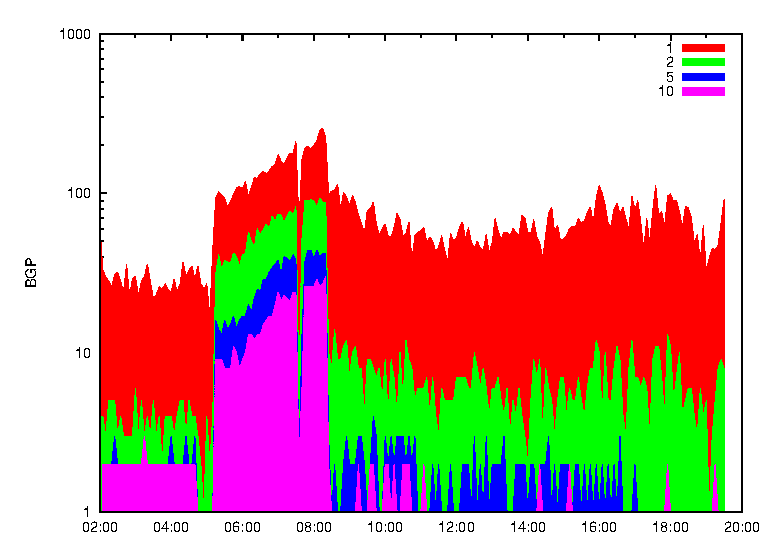
\includegraphics[width=0.75\linewidth]{images/events/2010_03_25/bgp_log_port80_ref.eps} \caption{Event 1: Unreachable \gls{bgp} prefixes detected by the classical \gls{FACT} traffic preselection based on the port-based heuristic.} 
	\label{fig:AMS_IX_FACT_REF} 
\end{figure}

\subsubsection{Server Socket Approach}

Firstly, \gls{FACT}s results of set \emph{C}, containing all detected port 80 \glspl{server socket} are inspected. 
This socket set can directly be compared to the old heuristic approach, since it monitors a majority of the legitimate traffic to port 80 as well. 

As figure \ref{fig:AMS_IX_FACT_allSES80} shows, the real event lasting from 05.00 UTC to 08:15 UTC is clearly visible equally well as in the heuristic approach from figure \ref{fig:AMS_IX_FACT_REF}. 
However, the \gls{server socket} based approach reduces the red part indicating the number of unreachable prefixes affecting only a single internal user by at least an order of magnitude. 
Hence, the event is now clearly standing out of the \emph{background event detection noise} -- the green and red part of figure \ref{fig:AMS_IX_FACT_REF}. 

Despite the fact that the set \emph{C} is not optimized at all with respect to stability, popularity and visibility, it outperforms the traditional approach in terms of noise reduction without significantly worsen the actual event detection. 
This confirms the assumption that a high number of unreachable prefixes affecting only a single internal user is caused by malware and \gls{p2p} churn.

Comparing the results from set \emph{C} to those from set \emph{D} which limits the sockets by only selecting the sockets seen at least at two days, yields almost no visual difference between figure \ref{fig:AMS_IX_FACT_allSES80VTS2} and \ref{fig:AMS_IX_FACT_allSES80}, despite the number of sockets is reduced by almost a third. 
However, if also the stability is considered as by set \emph{E}, the red and green noise can be further reduced without significantly affecting the blue and pink part of the event.

If the \glspl{server socket} are not anymore artificially constrained to be a port 80 \gls{server socket} as in the case of set \emph{A} and \emph{B}, there is a clear increase of unreachable sockets visible in figure \ref{fig:AMS_IX_FACT_allSES} with all server sockets and even in figure \ref{fig:AMS_IX_FACT_popularVTS2STAB9}. 
The original \gls{FACT} detects up to 30 unreachable prefixes with 10 or more internal users affected, \gls{FACT} with set \emph{A} and \emph{B} detect up to 112, respectively up to 72 distinct unreachable prefixes. 
Remarkable is that the red and green part of figure \ref{fig:AMS_IX_FACT_allSES} and \ref{fig:AMS_IX_FACT_popularVTS2STAB9} are significantly lower than in the case of the original results from figure \ref{fig:AMS_IX_FACT_REF}. 
\begin{figure}
	[p] \centering 
	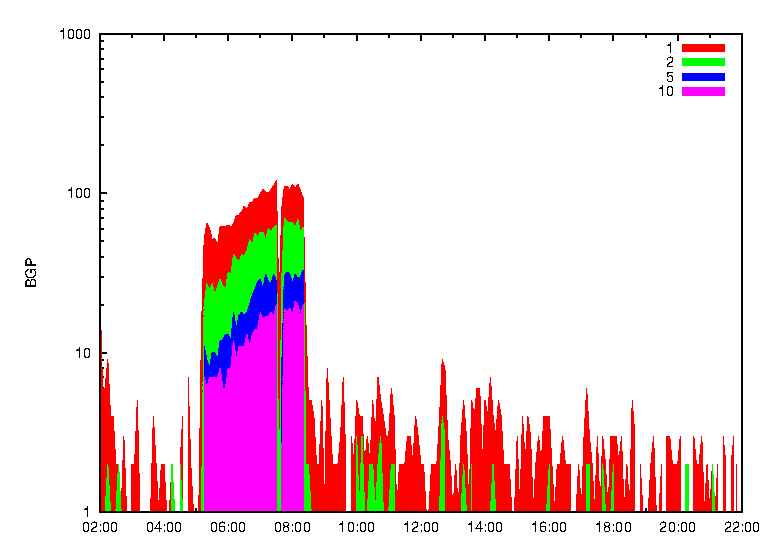
\includegraphics[width=0.75\linewidth]{images/events/2010_03_25/bgp_log_allPort80SES.eps} \caption{Event 1: Unreachable \gls{bgp} prefixes detected by the modified \gls{FACT} traffic preselection based on all port 80 \glspl{server socket}.} 
	\label{fig:AMS_IX_FACT_allSES80} 
\end{figure}
\begin{figure}
	[p] \centering 
	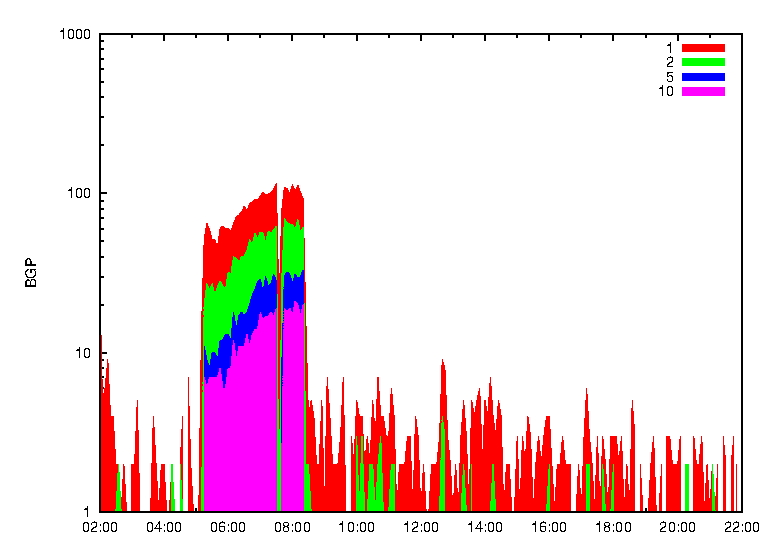
\includegraphics[width=0.75\linewidth]{images/events/2010_03_25/bgp_log_port80_Set_stab_0_vts_2.eps} \caption{Event 1: Unreachable \gls{bgp} prefixes detected by the modified \gls{FACT} traffic preselection based on all port 80 \glspl{server socket} with visibility of at least 2 days.} 
	\label{fig:AMS_IX_FACT_allSES80VTS2} 
\end{figure}
\begin{figure}
	[p] \centering 
	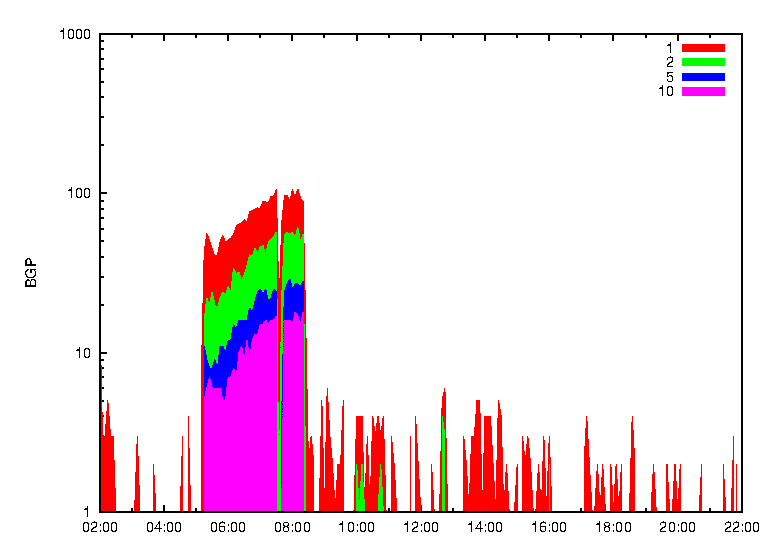
\includegraphics[width=0.75\linewidth]{images/events/2010_03_25/bgp_log_port80_Set_stab_9_vts_2.eps} \caption{Event 1: Unreachable \gls{bgp} prefixes detected by the modified \gls{FACT} traffic preselection based on all port 80 \glspl{server socket} with visibility of at least 2 days and stability ratio of at least $90\%$.} 
	\label{fig:AMS_IX_FACT_allSES80VTS2STAB9} 
\end{figure}
\begin{figure}
	[p] \centering 
	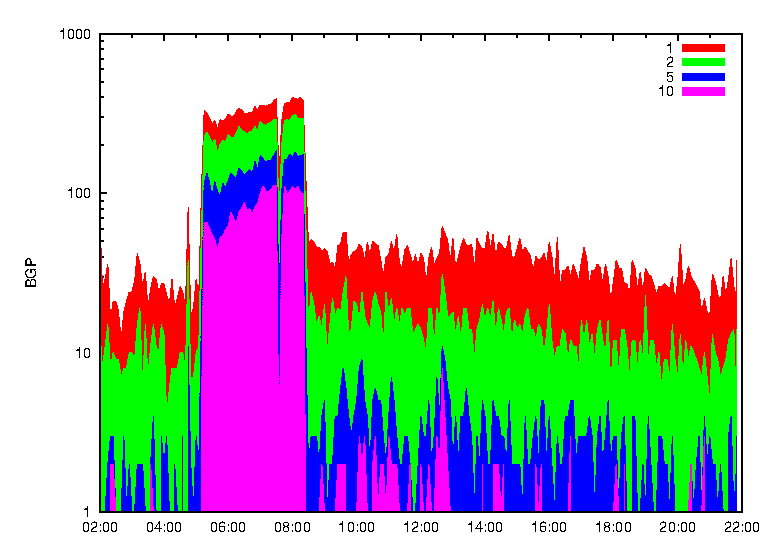
\includegraphics[width=0.75\linewidth]{images/events/2010_03_25/bgp_log_all_external.eps} \caption{Event 1: Unreachable \gls{bgp} prefixes detected by the modified \gls{FACT} traffic preselection based on all detected \glspl{server socket}} 
	\label{fig:AMS_IX_FACT_allSES} 
\end{figure}
\begin{figure}
	[p] \centering 
	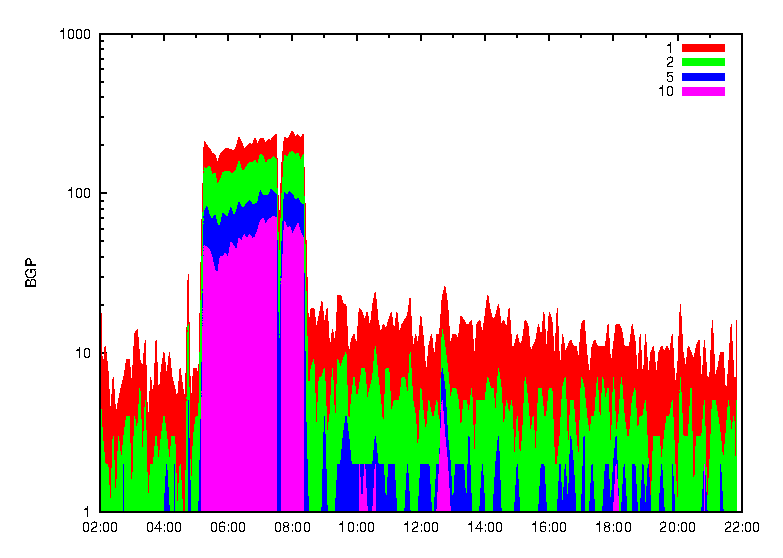
\includegraphics[width=0.75\linewidth]{images/events/2010_03_25/bgp_log_Set_var_0_1_stab_9_vts_2.eps} \caption{Event 1: Unreachable \gls{bgp} prefixes detected by the modified \gls{FACT} traffic preselection based on the $70\%$ most popular \glspl{server socket} limited to those with a visibility of at least 2 days and stability ratio of at least $90\%$.} 
	\label{fig:AMS_IX_FACT_popularVTS2STAB9} 
\end{figure}

%%%%%%%%%%%%%%%%%%%%%%%%%%%%%%%%%%%%%%%%%%%%%%%%%%%%%%%%%%%%%%%%%%%%%%%%%%%%%%%%
% EVENT 2: TIER-1 BLACK-HOLING
%%%%%%%%%%%%%%%%%%%%%%%%%%%%%%%%%%%%%%%%%%%%%%%%%%%%%%%%%%%%%%%%%%%%%%%%%%%%%%%%
\newpage 
\subsection{Event 2: Reverse Path Traffic Black-holing}

On May 18, 2010, the operators of the SWITCH network were assigned to investigate an reported issue that all services in an external /24 network were not accessible from the SWITCH network between 08:30 and 08:45 UTC. 
According to SWITCH, the problem was most likely due to an issue of an tier-1 provider which black-holed parts of the reverse traffic towards the SWITCH network\citep{SchatzmannPAM2011}.

Unfortunately, the operators were neither able to tell how many internal users were affected nor how many external networks were unreachable during this period of time. 
However with the help of \gls{FACT}, this issue can be further assessed with respect to the severity of the event\citep{SchatzmannPAM2011}.

\subsubsection{Heuristic Approach}

Figure \ref{fig:TIER1_FACT_REF} illustrates the unreachable prefixes detected by the port-based heuristic of \gls{FACT}. 
The event is indeed visible around 08:30 UTC until 08:45 UTC as a high pink peak. 
There are 12 external unreachable prefixes affecting more than 10 internal users. 
Furthermore, a strong diurnal pattern of the red and green area is visible in figure \ref{fig:TIER1_FACT_REF}. 
\begin{figure}
	[p] \centering 
	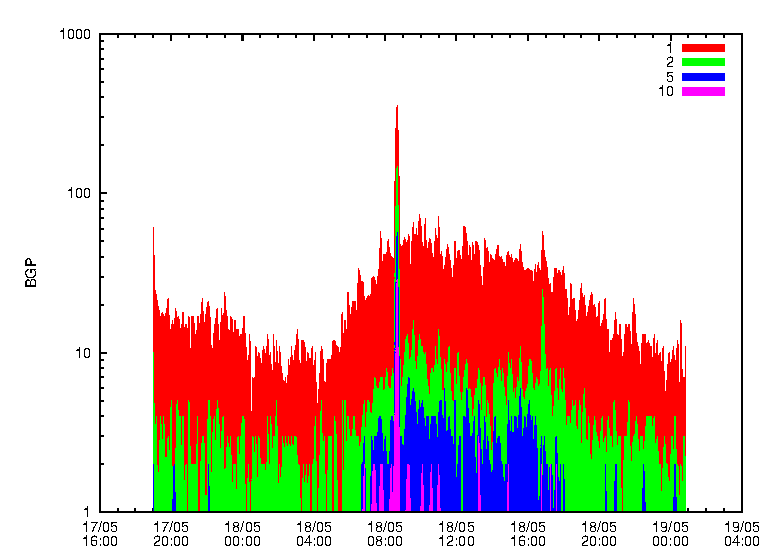
\includegraphics[width=0.75\linewidth]{images/events/2010_05_18/bgp_log_port80_ref.eps} \caption{Event 2: Unreachable \gls{bgp} prefixes detected by the classical \gls{FACT} traffic preselection based on the port-based heuristic.} 
	\label{fig:TIER1_FACT_REF} 
\end{figure}

\subsubsection{Server Socket Approach}

Again, the results of set \emph{C} which contains all port 80 \glspl{server socket} are directly comparable to the port-based heuristic approach. 
As figure \ref{fig:TIER1_FACT_allSES80} shows that the noise of the red and green area is reduced by at least an order of magnitude without worsen the real event detection at all.

Considering the visibility of the sockets as done by set \emph{D}, does not significantly change the visual appearance of the event at all as depicted by figure \ref{fig:TIER1_FACT_allSES80VTS2}. 
However, if the stability is considered as well by set \emph{E}, the noise can be even further reduced. 

By extending the set to all detected \glspl{server socket} (set \emph{A}), an increase of the unreachable prefixes by almost a factor of 6 is visible in figure \ref{fig:TIER1_FACT_allSES}. 
However, also the noise is increased, but still lower than the reference result from the port-based heuristic approach. 

By comparing figure \ref{fig:TIER1_FACT_allSES} with \ref{fig:TIER1_FACT_popularVTS2STAB9}, it becomes obvious that restricting the socket set by popularity, visibility and stability characteristics (set \emph{B}) does minimize the noise again by almost an order of magnitude with respect to all \glspl{server socket}. 
Additionally, it is remarkable that the diurnal pattern is less marked than in figure \ref{fig:TIER1_FACT_REF}. 
Though, no clear reason for this is identifiable. 
\begin{figure}
	[p] \centering 
	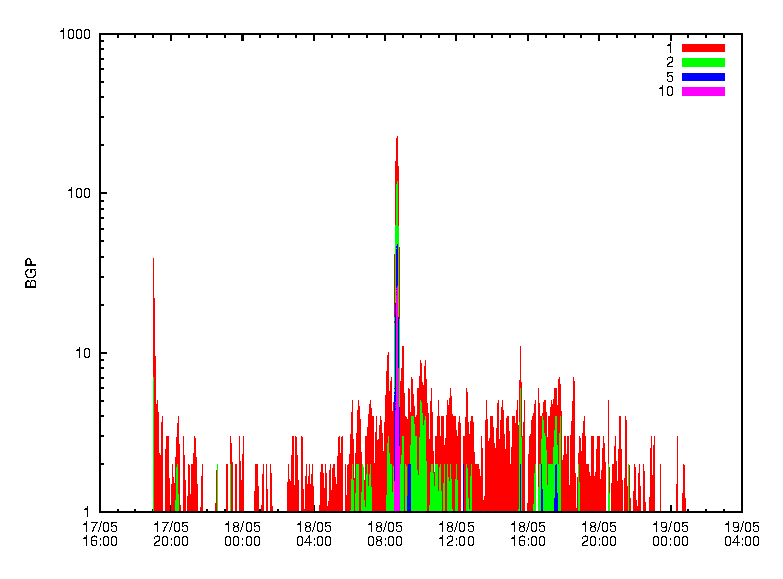
\includegraphics[width=0.75\linewidth]{images/events/2010_05_18/bgp_log_allPort80SES.eps} \caption{Event 2: Unreachable \gls{bgp} prefixes detected by the modified \gls{FACT} traffic preselection based on all port 80 \glspl{server socket}.} 
	\label{fig:TIER1_FACT_allSES80} 
\end{figure}
\begin{figure}
	[p] \centering 
	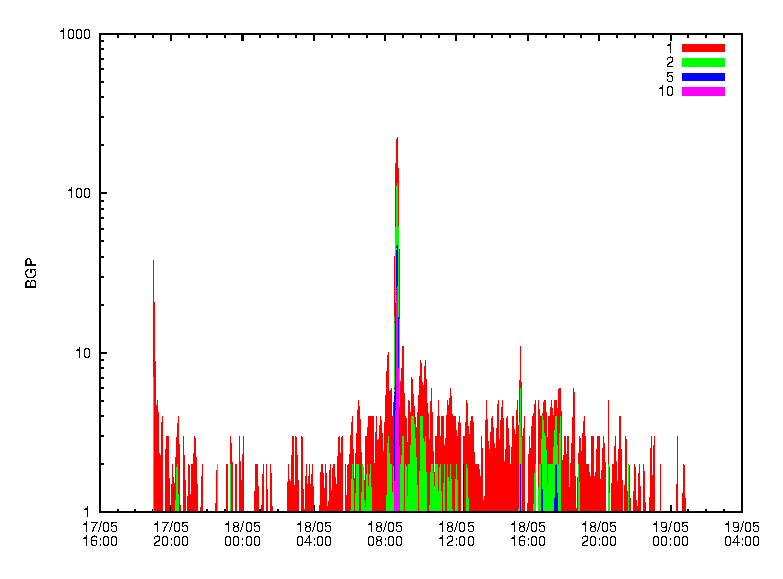
\includegraphics[width=0.75\linewidth]{images/events/2010_05_18/bgp_log_port80_Set_stab_0_vts_2.eps} \caption{Event 2: Unreachable \gls{bgp} prefixes detected by the modified \gls{FACT} traffic preselection based on all port 80 \glspl{server socket} with visibility of at least 2 days.} 
	\label{fig:TIER1_FACT_allSES80VTS2} 
\end{figure}
\begin{figure}
	[p] \centering 
	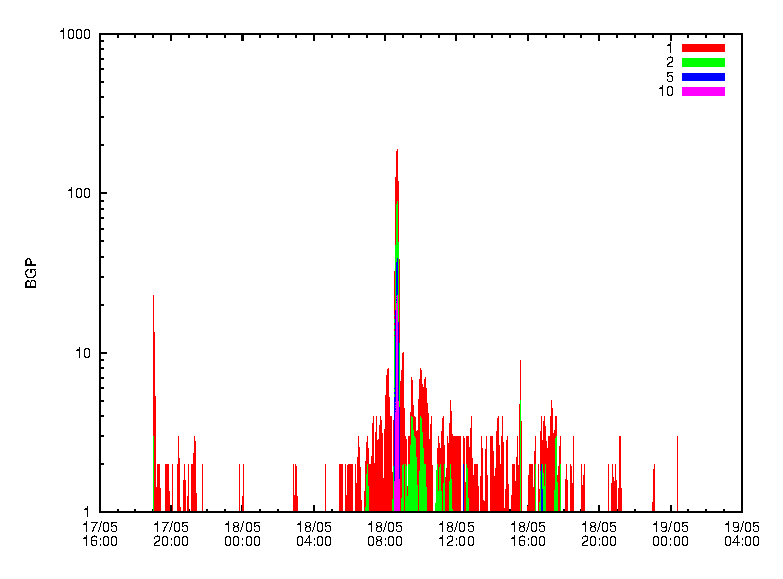
\includegraphics[width=0.75\linewidth]{images/events/2010_05_18/bgp_log_port80_Set_stab_9_vts_2.eps} \caption{Event 2: Unreachable \gls{bgp} prefixes detected by the modified \gls{FACT} traffic preselection based on all port 80 \glspl{server socket} with visibility of at least 2 days and stability ratio of at least $90\%$.} 
	\label{fig:TIER1_FACT_allSES80VTS2STAB9} 
\end{figure}
\begin{figure}
	[p] \centering 
	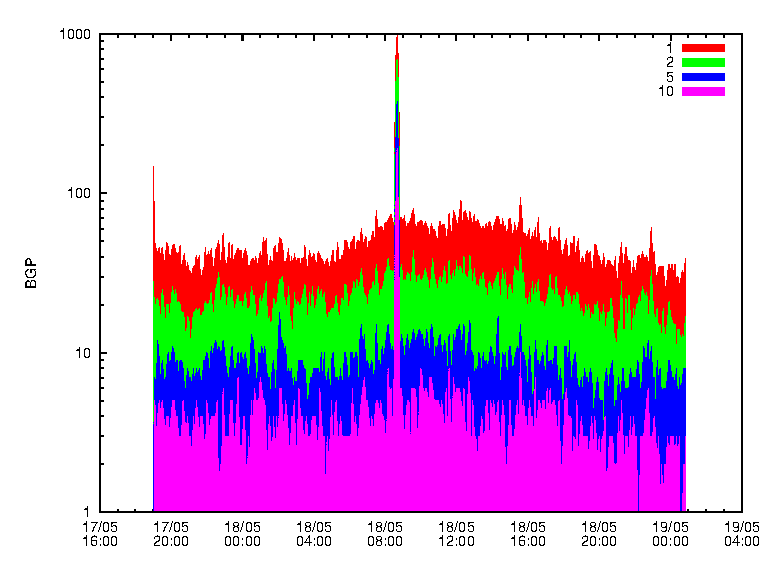
\includegraphics[width=0.75\linewidth]{images/events/2010_05_18/bgp_log_all_external.eps} \caption{Event 2: Unreachable \gls{bgp} prefixes detected by the modified \gls{FACT} traffic preselection based on all detected \glspl{server socket}} 
	\label{fig:TIER1_FACT_allSES} 
\end{figure}
\begin{figure}
	[p] \centering 
	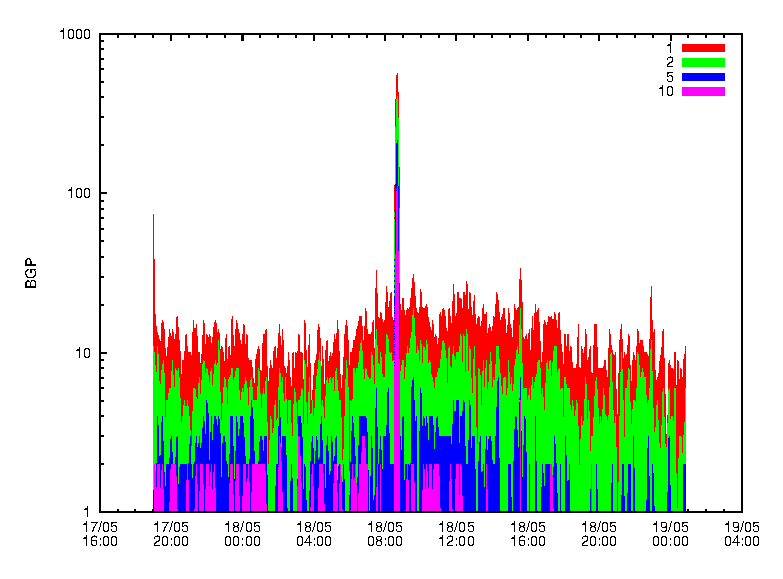
\includegraphics[width=0.75\linewidth]{images/events/2010_05_18/bgp_log_Set_var_0_1_stab_9_vts_2.eps} \caption{Event 2: Unreachable \gls{bgp} prefixes detected by the modified \gls{FACT} traffic preselection based on the $70\%$ most popular \glspl{server socket} limited to those with a visibility of at least 2 days and stability ratio of at least $90\%$.} 
	\label{fig:TIER1_FACT_popularVTS2STAB9} 
\end{figure}

%%%%%%%%%%%%%%%%%%%%%%%%%%%%%%%%%%%%%%%%%%%%%%%%%%%%%%%%%%%%%%%%%%%%%%%%%%%%%%%%
% EVENT 3: RIPE / DUKE BGP EXPERIMENT
%%%%%%%%%%%%%%%%%%%%%%%%%%%%%%%%%%%%%%%%%%%%%%%%%%%%%%%%%%%%%%%%%%%%%%%%%%%%%%%%
\newpage 
\subsection{Event 3: RIPE / DUKE BGP Experiments}

An experiment with new \gls{bgp} attributes jointly performed by RIPE and the Duke University on August 27, 2010, resulted in several unreachable prefixes\citep{SchatzmannPAM2011}. 
These new kind of attributes have never been announced on the Internet before, although the were in accordance with the \gls{bgp} specification\citep{ripe_duke}.

These new kind of attributes uncovered and triggered a bug in some Cisco router known as the \emph{Cisco IOS XR Software Border Gateway Protocol Vulnerability (SA-20100827-BGP)}\citep{cisco_vulnerability}. 
In particular, the announcements with the new attributes were corrupted by the Cisco routers and send to their peers. 
Consequently, their peers detected the corruption and dropped the entire peering session\citep{ripe_duke}.

\subsubsection{Heuristic Approach} Figure \ref{fig:RIPE_FACT_REF} shows the unreachable prefixes over time from August 26 2010 and August 27 2010. 
The RIPE / DUKE BGP experiment is well visible in the results of \gls{FACT} from August 27 2010 08:50 UTC until 09:10 UTC with up to 3 unreachable prefixes affecting more than 10 internal users. 

The port-based heuristic approach of \gls{FACT} does report a high number of unreachable \gls{bgp} prefixes as unreachable affecting only one or two internal clients and showing a strong diurnal pattern thereof. 
\begin{figure}
	[p] \centering 
	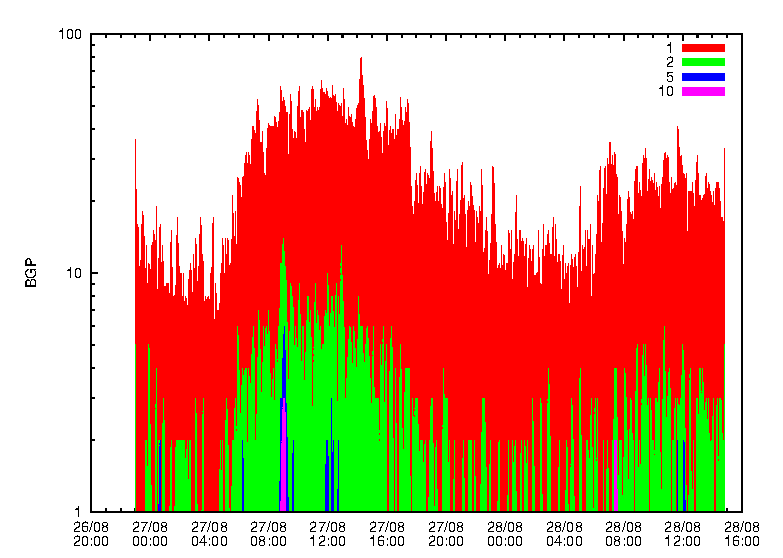
\includegraphics[width=0.75\linewidth]{images/events/2010_08_27/bgp_log_port80_ref.eps} \caption{Event 3: Unreachable \gls{bgp} prefixes detected by the classical \gls{FACT} traffic preselection based on the port-based heuristic.} 
	\label{fig:RIPE_FACT_REF} 
\end{figure}

\subsubsection{Server Socket Approach} 

By comparing figure \ref{fig:RIPE_FACT_REF} with figure \ref{fig:RIPE_FACT_allSES80} it becomes obvious that the \gls{server socket} based approach of figure \ref{fig:RIPE_FACT_allSES80} reduces the red and green area by an order of magnitude without restrain the visibility of the real event shown in pink from 08:50 to 09:10 UTC. 
The adjusted traffic selection of \gls{FACT} yields exactly the same unreachable prefixes as the original port-based heuristic approach. 
Constraining set \emph{C} by the visible days of the sockets does not improve the noise reduction as figure \ref{fig:RIPE_FACT_allSES80VTS2} shows. 
However, the number of sockets of set \emph{D} is reduced by around a third, thus allowing a faster processing.

If as in case of set \emph{E} also the stability is considered, the noise is again reduced, although also at the cost of the event visibility. 
As figure \ref{fig:RIPE_FACT_allSES80VTS2STAB9}, \gls{FACT} is detecting only 2 unreachable prefixes affecting more than 10 internal users and hence, clearly missing one unreachable prefix. 

On the contrary, if \gls{FACT} is using set \emph{A}, it is able to reveal almost up to 20 unreachable prefixes affecting more than 10 internal users. 
Though, this comes at the cost of a even bigger red area than in case of the original port 80 based approach as it can be seen in figure \ref{fig:RIPE_FACT_allSES}. 
Luckily, as figure \ref{fig:RIPE_FACT_popularVTS2STAB9} shows \gls{FACT} is able to detect up to 14 distinct unreachable prefixes even with the smallest socket set. 
Moreover, also the noise is considerably reduced compared to the port 80 based approach shown in figure \ref{fig:RIPE_FACT_REF}.
\begin{figure}
	[p] \centering 
	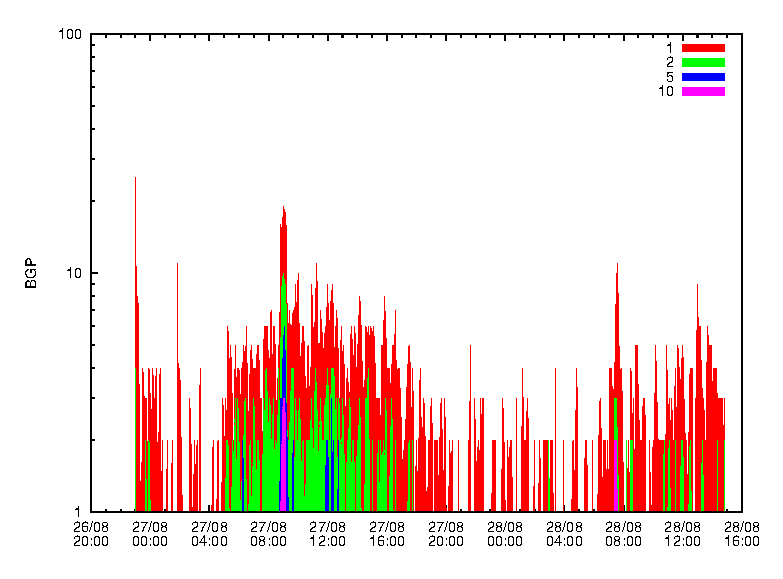
\includegraphics[width=0.75\linewidth]{images/events/2010_08_27/bgp_log_allPort80SES.eps} \caption{Event 3: Unreachable \gls{bgp} prefixes detected by the modified \gls{FACT} traffic preselection based on all port 80 \glspl{server socket}.} 
	\label{fig:RIPE_FACT_allSES80} 
\end{figure}
\begin{figure}
	[p] \centering 
	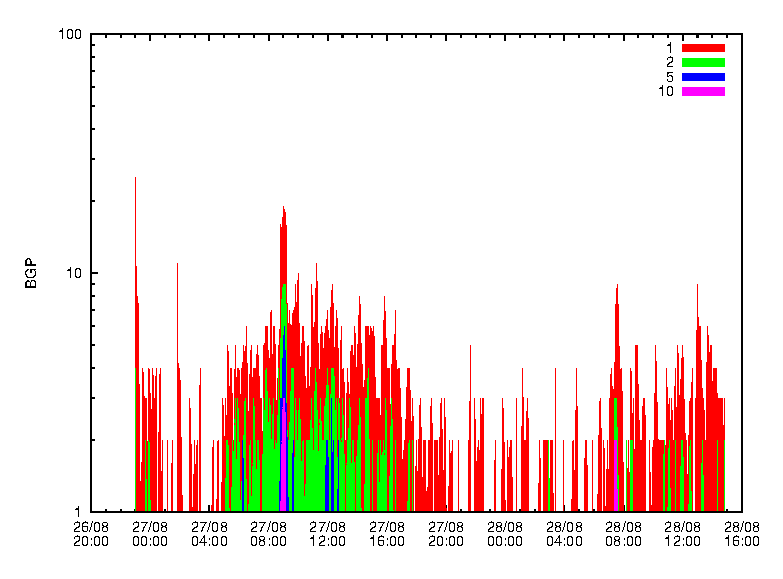
\includegraphics[width=0.75\linewidth]{images/events/2010_08_27/bgp_log_port80_Set_stab_0_vts_2.eps} \caption{Event 3: Unreachable \gls{bgp} prefixes detected by the modified \gls{FACT} traffic preselection based on all port 80 \glspl{server socket} with visibility of at least 2 days.} 
	\label{fig:RIPE_FACT_allSES80VTS2} 
\end{figure}
\begin{figure}
	[p] \centering 
	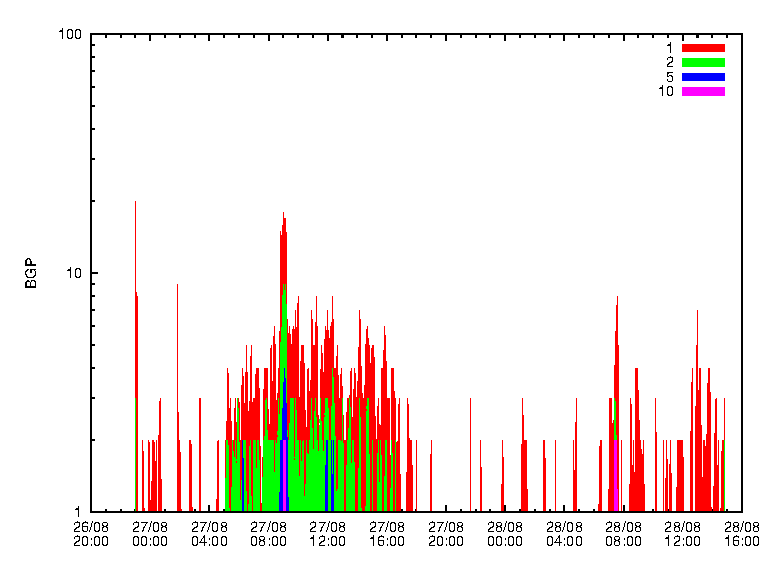
\includegraphics[width=0.75\linewidth]{images/events/2010_08_27/bgp_log_port80_Set_stab_9_vts_2.eps} \caption{Event 3: Unreachable \gls{bgp} prefixes detected by the modified \gls{FACT} traffic preselection based on all port 80 \glspl{server socket} with visibility of at least 2 days and stability ratio of at least $90\%$.} 
	\label{fig:RIPE_FACT_allSES80VTS2STAB9} 
\end{figure}
\begin{figure}
	[p] \centering 
	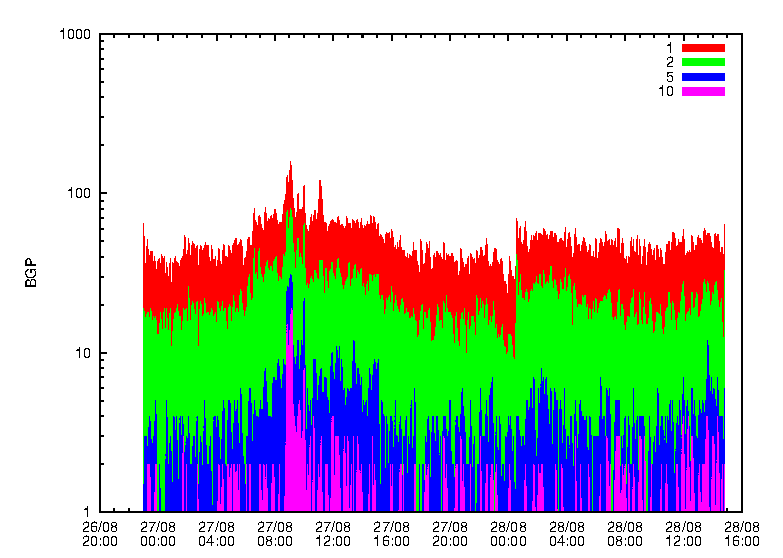
\includegraphics[width=0.75\linewidth]{images/events/2010_08_27/bgp_log_all_external.eps} \caption{Event 3: Unreachable \gls{bgp} prefixes detected by the modified \gls{FACT} traffic preselection based on all detected \glspl{server socket}} 
	\label{fig:RIPE_FACT_allSES} 
\end{figure}
\begin{figure}
	[p] \centering 
	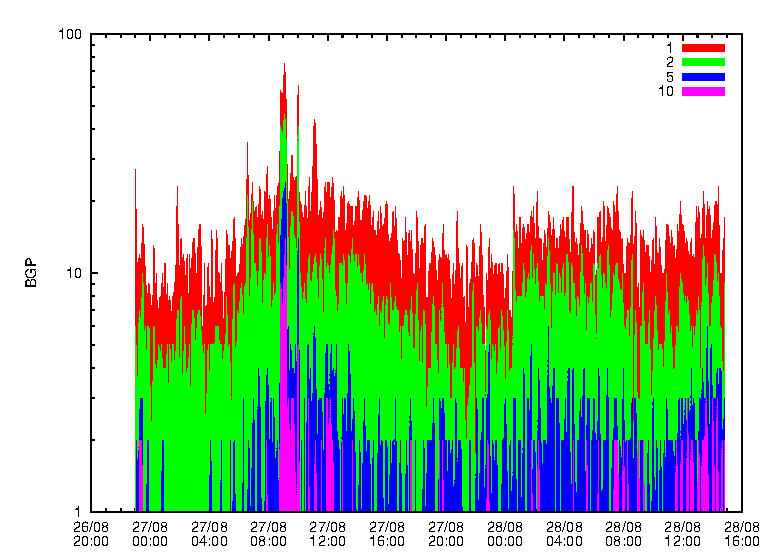
\includegraphics[width=0.75\linewidth]{images/events/2010_08_27/bgp_log_Set_var_0_1_stab_9_vts_2.eps} \caption{Event 3: Unreachable \gls{bgp} prefixes detected by the modified \gls{FACT} traffic preselection based on the $70\%$ most popular \glspl{server socket} limited to those with a visibility of at least 2 days and stability ratio of at least $90\%$.} 
	\label{fig:RIPE_FACT_popularVTS2STAB9} 
\end{figure}

%%%%%%%%%%%%%%%%%%%%%%%%%%%%%%%%%%%%%%%%%%%%%%%%%%%%%%%%%%%%%%%%%%%%%%%%%%%%%%%%
% RESULTS
%%%%%%%%%%%%%%%%%%%%%%%%%%%%%%%%%%%%%%%%%%%%%%%%%%%%%%%%%%%%%%%%%%%%%%%%%%%%%%%%
\newpage 
\section{Results\label{section:results}} 
Generally, \gls{FACT}s results of the \gls{server socket} approach are better with almost all sets compared to the port 80 based heuristic. 
Though, there are significant differences between the results of the different \gls{server socket} sets. 

On the one side, constraining the sockets to be port 80 is good for comparing with the original approach, practically its too restrictive and as the comparison of the coverage from table \ref{tab:ses_sets_coverage} shows there is a better coverage with even less sockets possible. 
Thus, it is possible to get either a greater network visibility as well as a more diverse observation space. Especially in case of the RIPE/DUKE event, this produces a much better view of the event. 

On the other side, constraining the sockets by their characteristics of visibility, stability and popularity allows to minimize the number of sockets removing unsuitable sockets for connectivity tracking and thus, reducing the noise of the network outage event detection.

From the five evaluated \glspl{server socket} sets set \emph{D} have the least \glspl{server socket}, but provides a great visibility without generating to much noise.
Therefore, from the five evaluated sets, set \emph{D} is the best with respect to detection performance. 
However, as described previously the sets are chosen by manually comparing the network coverage and number of sockets, and thus, there may be other even better sets with respect to the detection performance. 
To find these sets the approach of selecting the sockets must be formally defined, e.g., as an optimization problem, and then adequately solved.

To sum up, the newly proposed approach of selecting the reflector traffic with the help of \glspl{server socket} actually decreases the detection noise and even provides a better event visibility and sensibility.
The performance of the approach is heavily influenced by the number of \glspl{server socket} which have to be considered during the generating of a good \gls{server socket} set.
Furthermore, this approach allows to better control the observation capabilities of \gls{FACT}, e.g., by completely excluding certain, uninteresting parts of the Internet from the observation scope.